\documentclass[a4paper,10pt,notitlepage]{scrartcl}

\usepackage[T1]{fontenc}
\usepackage[english]{babel}
\usepackage[utf8x]{inputenc}
\usepackage{setspace}
\usepackage{subfig}
\usepackage{textcomp}
\usepackage{graphicx}
\usepackage{fixltx2e}
\usepackage{multirow}
\usepackage{array}
\usepackage{amssymb}
\usepackage{amsmath}
\usepackage{subfig}
\usepackage{nomencl}
\usepackage[pdfborder={0 0 0}]{hyperref}
\usepackage{natbib}
% \usepackage{makeidx}
\usepackage{nicefrac}
\usepackage{bbold}
\usepackage{gensymb}
\usepackage{float}

\captionsetup{labelfont=footnotesize,textfont=footnotesize}

\newcolumntype{x}[1]{>{\begin{flushleft}$}p{#1}<{$\end{flushleft}}}
\newcolumntype{y}[1]{>{\begin{center}$}p{#1}<{$\end{center}}}
\newcolumntype{z}[1]{>{\begin{flushright}$}p{#1}<{$\end{flushright}}}
\newcolumntype{m}{>{$}l<{$}}
\newcolumntype{n}{>{$}c<{$}}
\newcolumntype{o}{>{$}r<{$}}

\newcommand{\mat}[1]{\mathbf{#1}} 

\bibliographystyle{plain}

% Title Page
\title{Scientific Visualization\\Project III}
\author{Milian Wolff}

\begin{document}
\maketitle

\begin{abstract}
In our fourth and last project for the the scientific visualization class
by Eugene Zhang we mainly investigated second order symmetric tensor fields.
Similar to the last exercise we write a JavaView based application that offers
an interface to design a tensor field using design elements. Furthermore we
extract degenerate points and visualize the separatrices.

The two other tasks in this project deepen our knowledge about vector field
topology by investigating the effects of a reverse stereographic projection.
Additionally we get acquainted with Conley indizes.

The source code of my exercise solutions can be found online under

\begin{center}\url{https://github.com/milianw/scivi}\end{center}
\end{abstract}

\begingroup
\let\clearpage\relax

\tableofcontents
\endgroup

\newpage

\section{Reverse Stereographic Projection}

Given a vector field $\vec{f}(x,y)$ in $R^2$ we project it onto the sphere
$S^2$. All three given vector fields have only a single singularity at $(x,y) =
(0,0)$, which corresponds to the South Pole on $S^2$. To have a well-defined
behavior of the field for $x,y \rightarrow \pm \infty$, we modify the magnitude
of the field without creating new singularities in $R^2$ by multiplying with a
scaling factor. This is just like we did in the last project for the vector
field design elements. Here we can use for example

\begin{equation}
 \sigma = \exp(-x^2-y^2).
\end{equation}

Through this modification we can safely apply the reverse stereographic
projection and will now always encounter a properly defined singularity at the
North Pole.

Since we know the euler characteristic of a sphere to be $\chi(S) = 2$, and
that this equals the sum of Poincar\`e-indizes $p_i$, i.e. $\chi(S) = 2 =
\sum p_i = p_{\text{NP}} + p_{\text{SP}}$, we find

\begin{equation}
  p_{\text{NP}} = 2 - p_{\text{SP}}.
\end{equation}

As such we can compute the Poincar\`e-index $p_{\text{NP}}$ at the North Pole
directly from the index $p_{\text{SP}}$ of the South Pole.

Note: To visualize the fields at the poles I wrote a small application,
\texttt{Ex4\_1}, which shows the field-direction. The higher-order design
elements, required to visualize the singularities at the North Pole can be
computed using eq. 10 from \cite{tfd},~p.~106, with $a = 1$, $b = 0$, $c = 0$,
$d = 1$, and $N = 2 \cdot p_{\text{NP}}$.

\subsection{Saddle}

The first vector field we investigate is that of a saddle:

\begin{equation}
 \vec{f} = \sigma \left( \begin{array}{c}
                   x \\ -y
                  \end{array} \right)
 \label{eq:vf-saddle}
\end{equation}

A saddle has an index $p = -1$. As such there will be a quadrupole at the North
Pole with an index of $p = 3$. See also fig. \ref{fig:vf-saddle} for images
of the field at both poles.

\begin{figure}[H]
  \centering
  \subfloat[Saddle at South Pole]{
    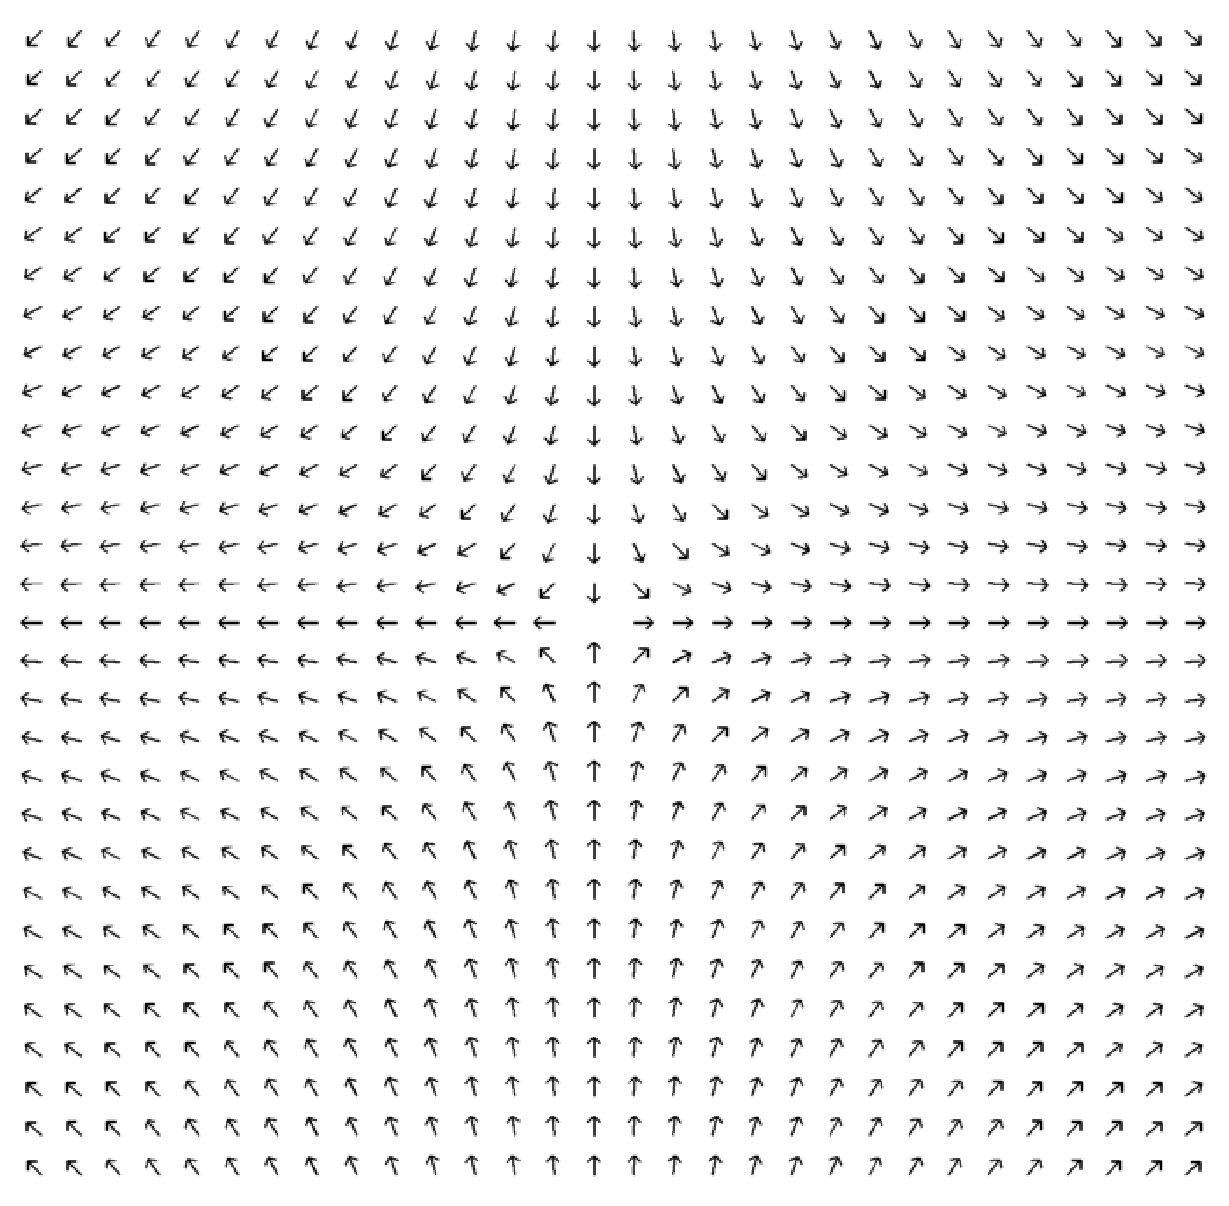
\includegraphics[width=0.4\textwidth]{img-4-2/f1-sp.eps}}
  \subfloat[Quadrupole at North Pole]{
    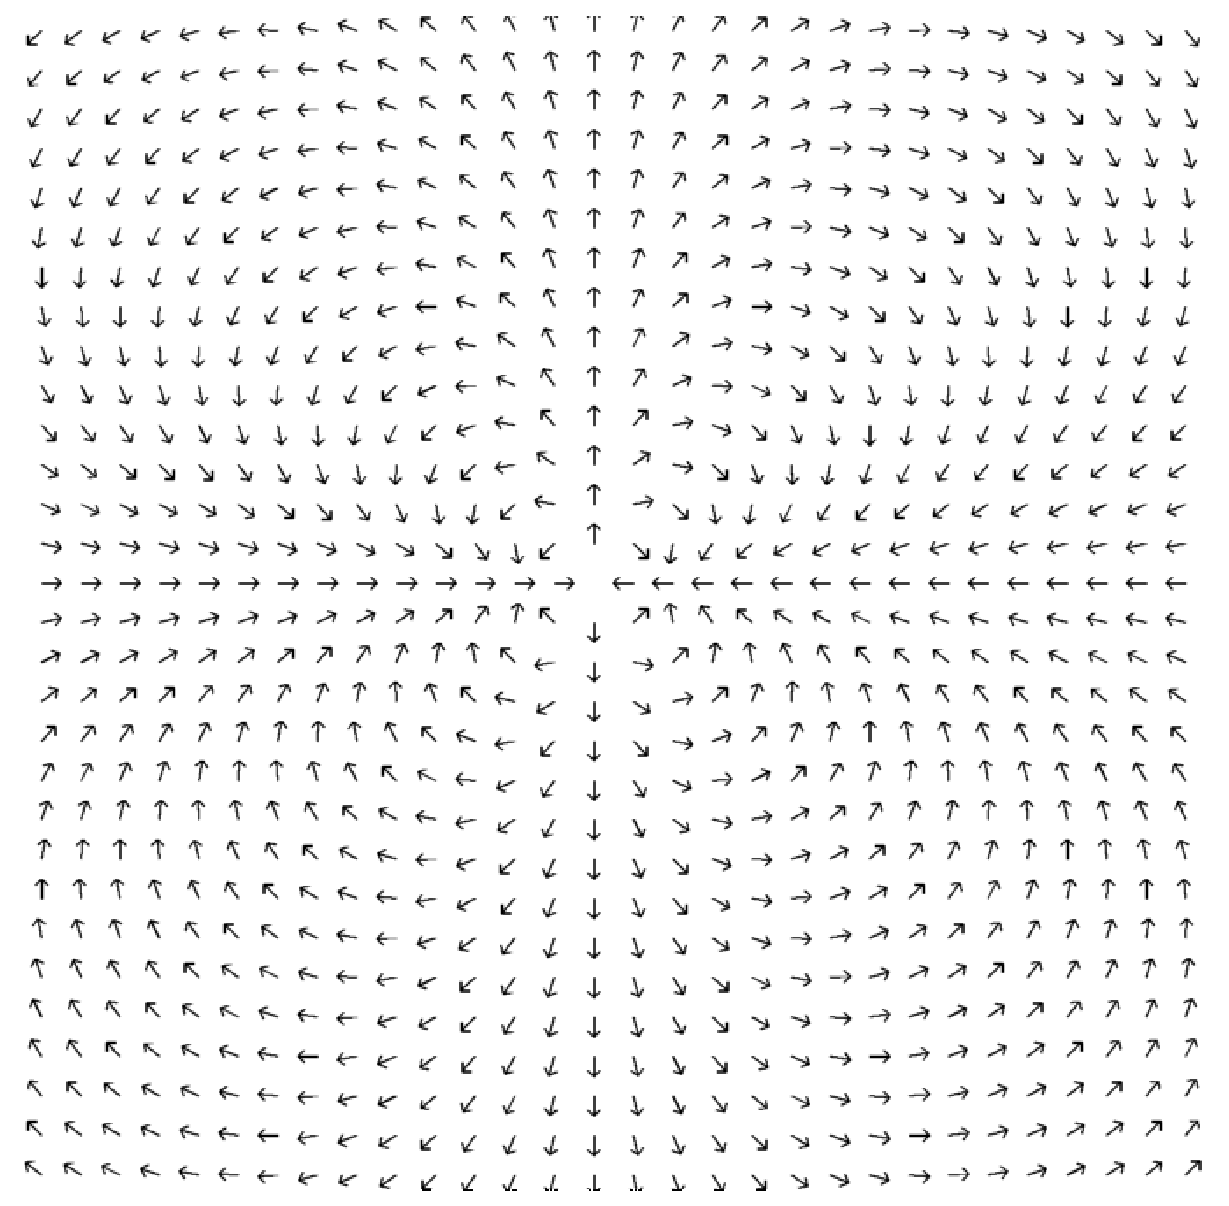
\includegraphics[width=0.4\textwidth]{img-4-2/f1-np.eps}}
  \caption{vector field from eq. \ref{eq:vf-saddle}}
  \label{fig:vf-saddle}
\end{figure}

\subsection{Monkey-Saddle}

The second vector field we investigate is that of a monkey-saddle:

\begin{equation}
 \vec{f} = \sigma \left( \begin{array}{c}
                   x^2-y^2 \\ -2xy
                  \end{array} \right)
 \label{eq:vf-monkey-saddle}
\end{equation}

A monkey-saddle has an index $p = -2$. As such there will be a hexapole at
the North Pole with an index of $p = 4$. See also fig.
\ref{fig:vf-monkey-saddle} for images of the field at both poles.

\begin{figure}[H]
  \centering
  \subfloat[Monkey-Saddle at South Pole]{
    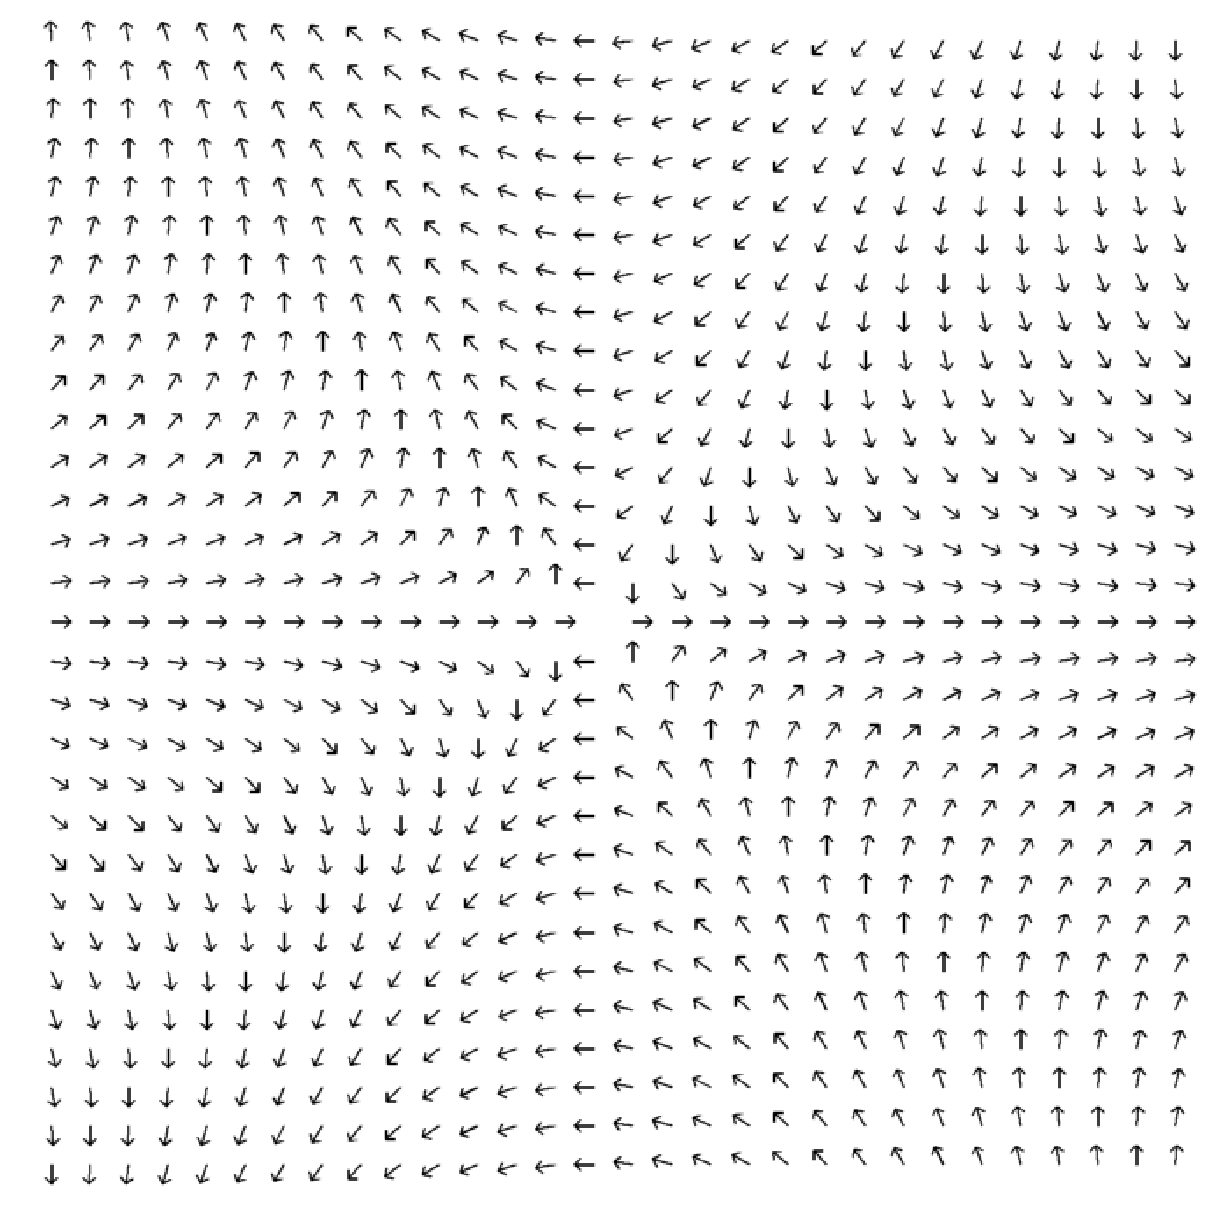
\includegraphics[width=0.4\textwidth]{img-4-2/f2-sp.eps}}
  \subfloat[Hexapole at North Pole]{
    \reflectbox{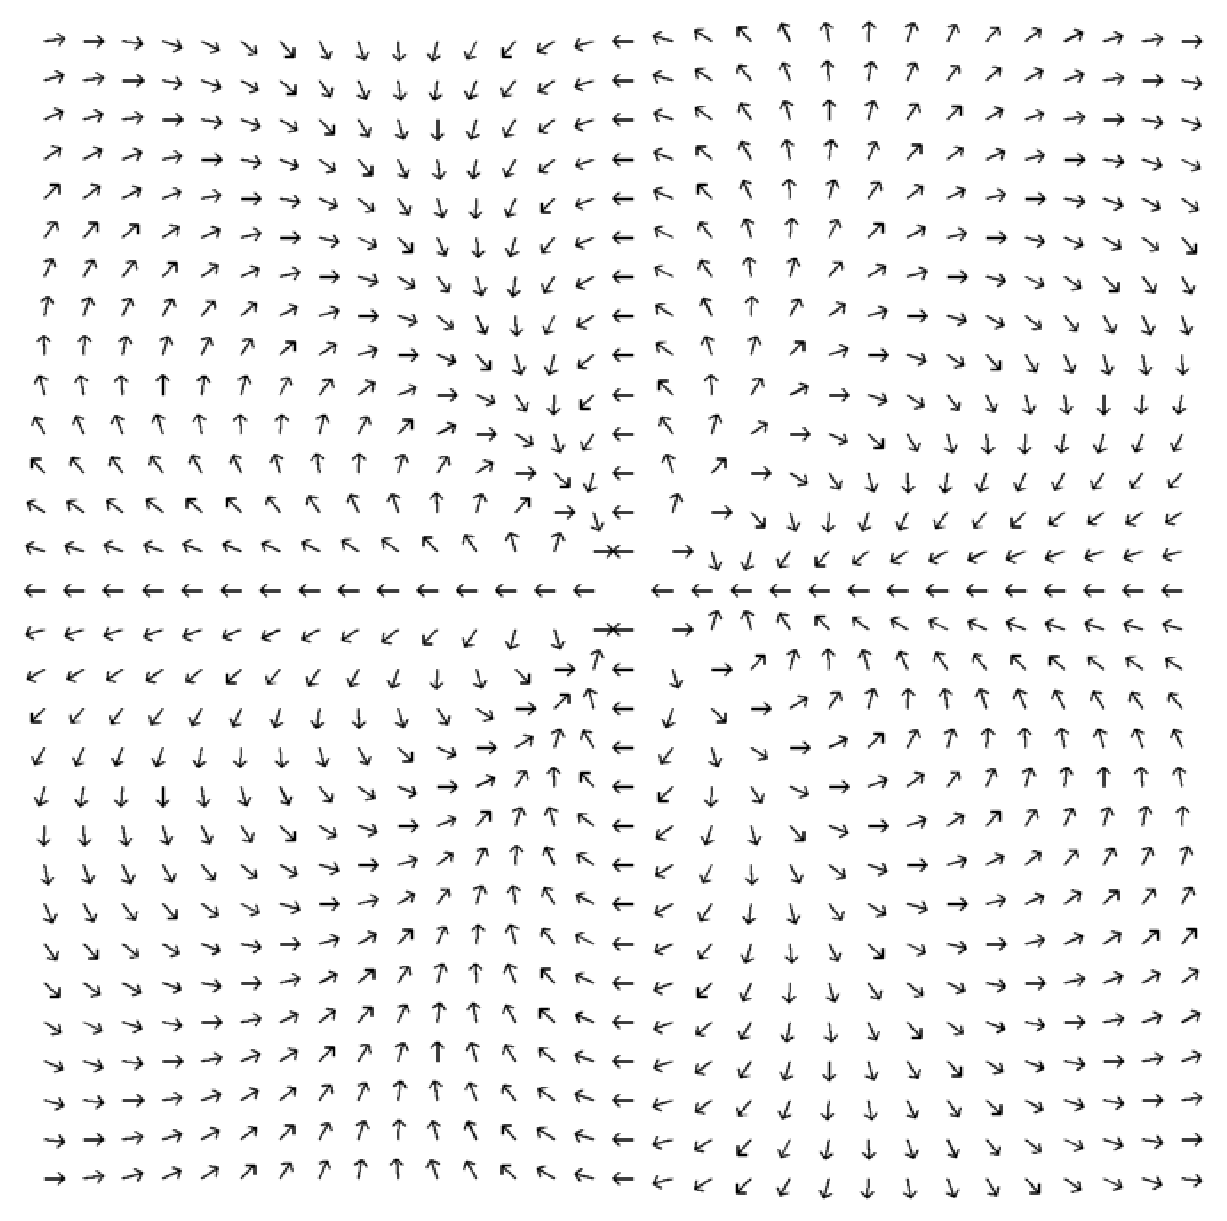
\includegraphics[width=0.4\textwidth]{img-4-2/f2-np.eps}}}
  \caption{vector field from eq. \ref{eq:vf-monkey-saddle}}
  \label{fig:vf-monkey-saddle}
\end{figure}

\subsection{Attractive CCW Rotation}

The third vector field represents an attractive clockwise rotation:

\begin{equation}
 \vec{f} = \sigma \left( \begin{array}{c}
                   x(1-\sqrt{x^2+y^2}) -y \\ x + y(1-\sqrt{x^2+y^2}
                  \end{array} \right)
 \label{eq:vf-rotation}
\end{equation}

Such a singularity has an index $p = 1$ and hence the singularity at the Nort
Pole will have the same index. Due to flow and symmetry conservation the
singularity must be a repulsive clockwise rotation. See also
\ref{fig:vf-rotation}.

\begin{figure}[H]
  \centering
  \subfloat[CCW-Rotation at South Pole]{
    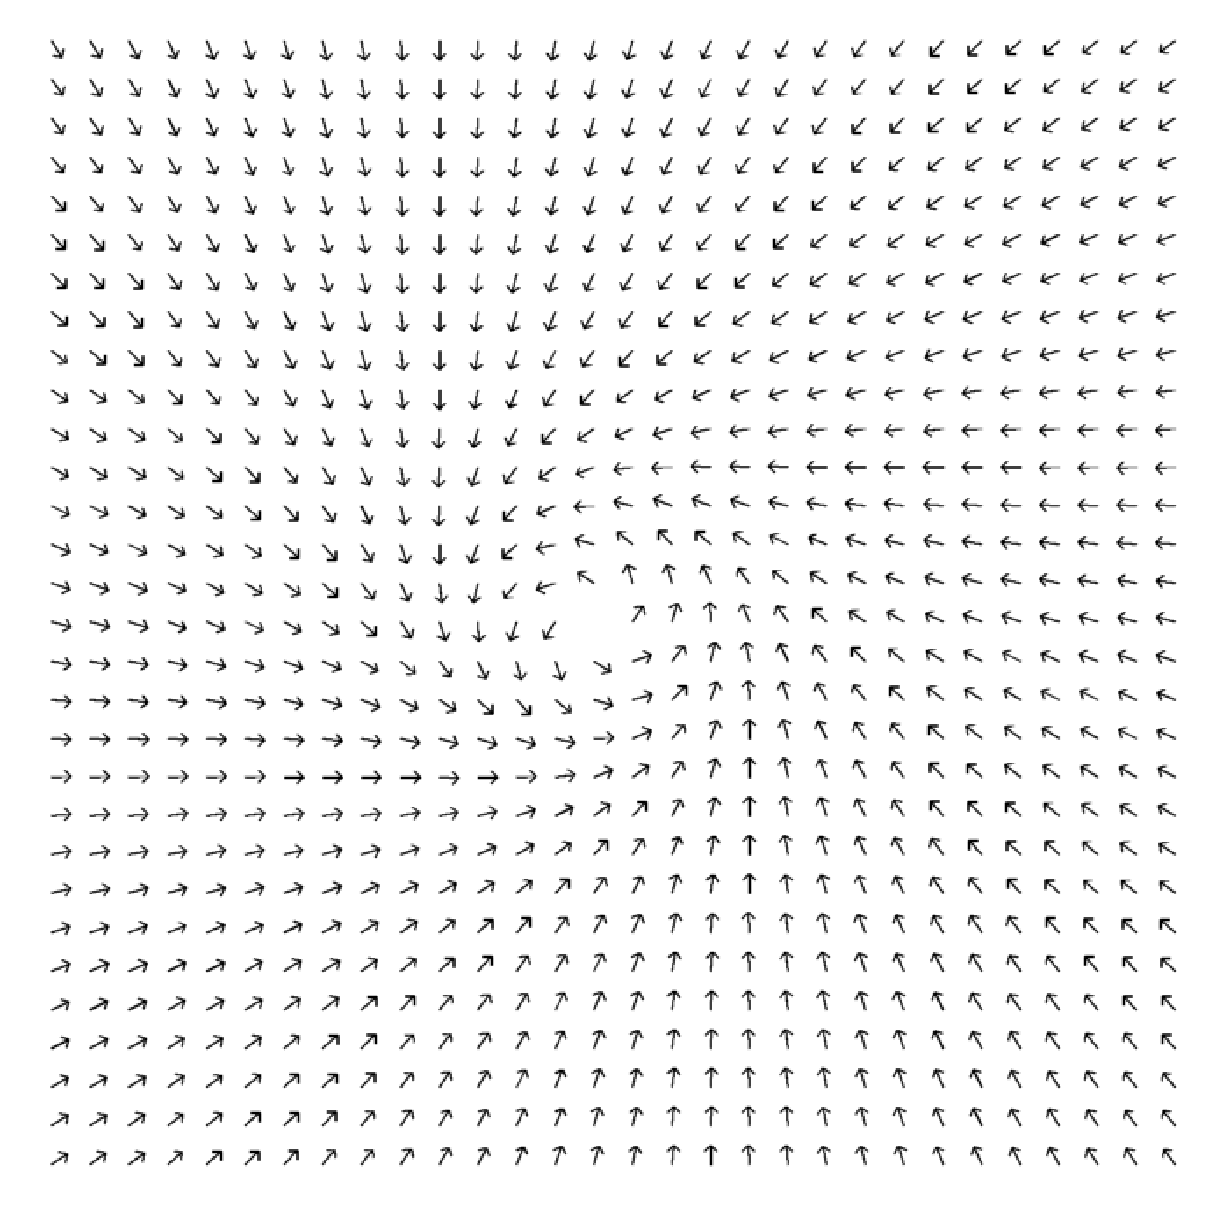
\includegraphics[width=0.4\textwidth]{img-4-2/f3-sp.eps}}
  \subfloat[CW-Rotation at North Pole]{
    \reflectbox{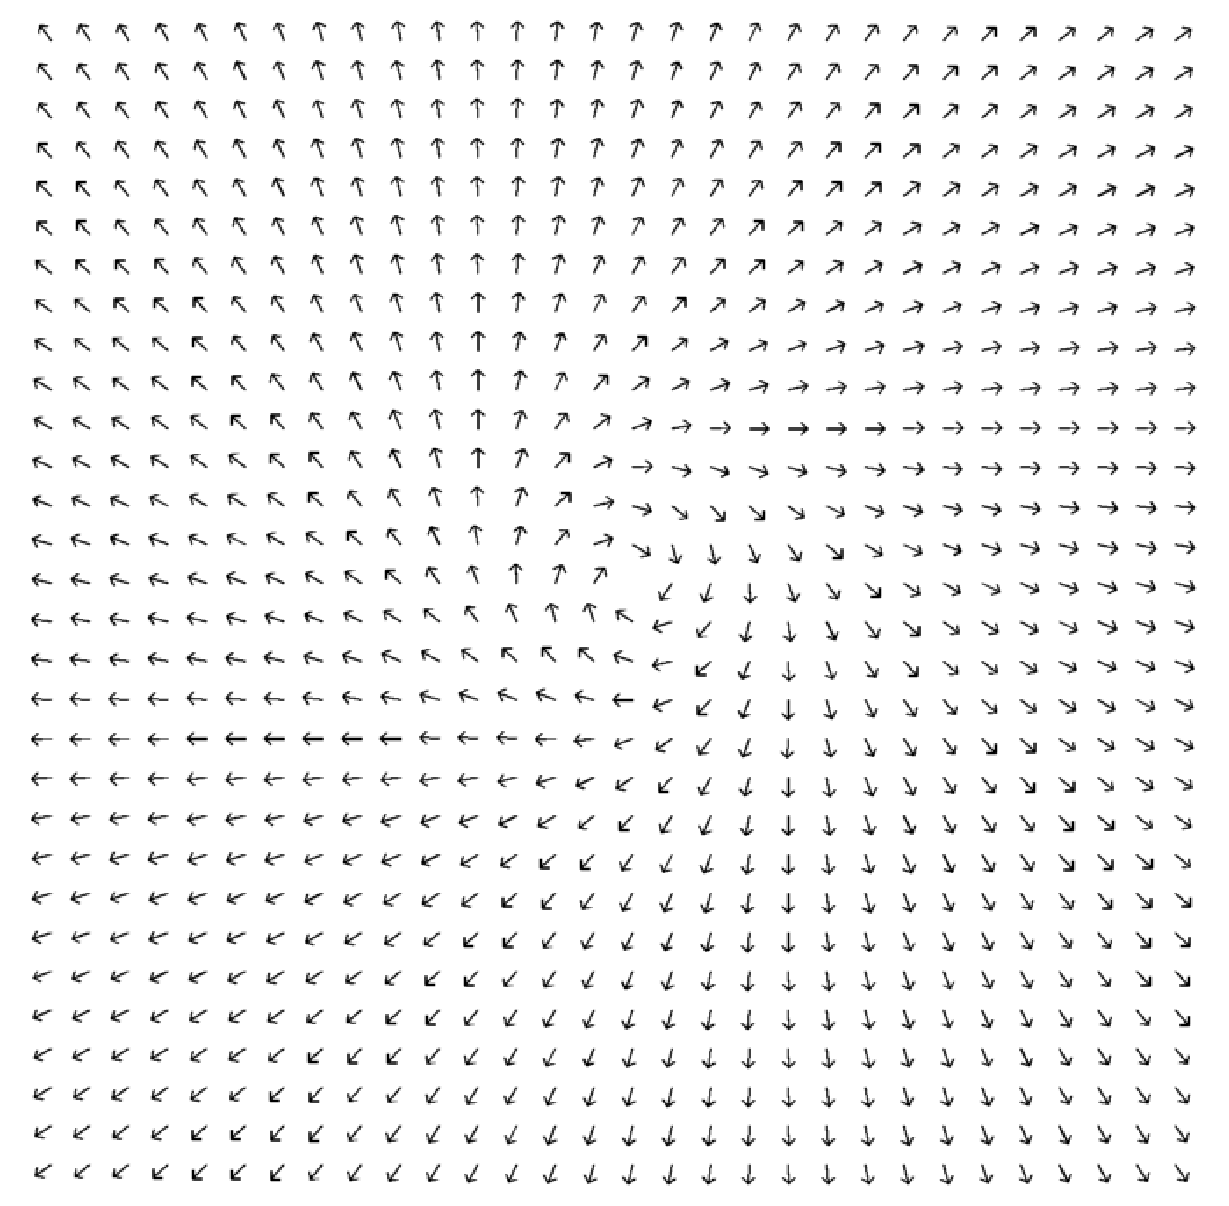
\includegraphics[width=0.4\textwidth]{img-4-2/f3-np.eps}}}
  \caption{vector field from eq. \ref{eq:vf-rotation}}
  \label{fig:vf-rotation}
\end{figure}

\section{Conley Indizes}

\subsection*{0, 0, 0}

Any vector field without a singularity will do the trick, see e.g. fig.
\ref{fig:conley-000}.

\begin{figure}
  \centering
  \subfloat{
    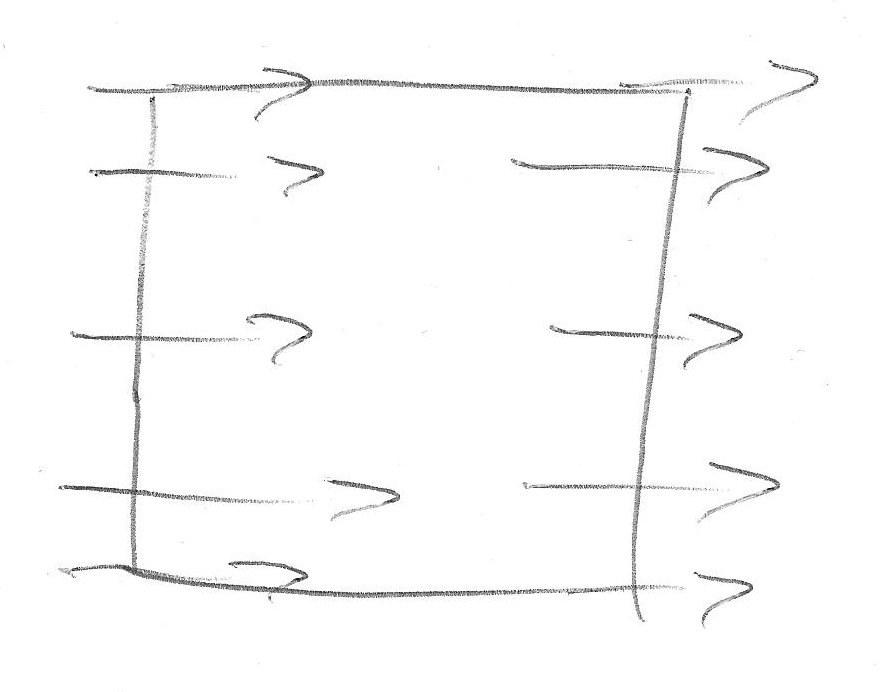
\includegraphics[width=0.4\textwidth]{img-4-2/conley-000-a.jpg}}
  \subfloat{
    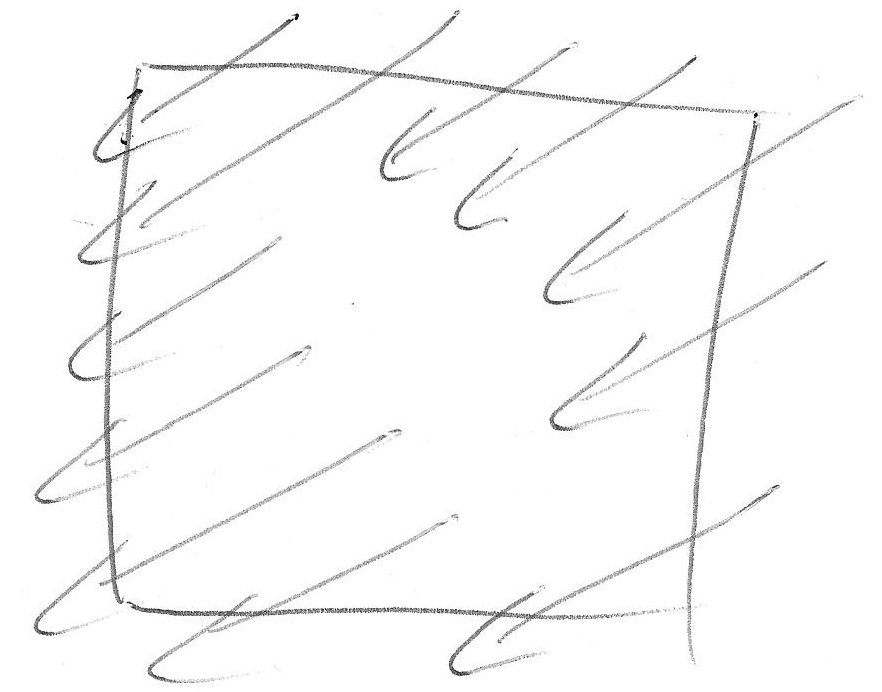
\includegraphics[width=0.4\textwidth]{img-4-2/conley-000-b.jpg}}
  \caption{vector fields for Conley index $\beta_0 = 0$, $\beta_1 = 0$ and
$\beta_2 = 0$}
  \label{fig:conley-000}
\end{figure}

\subsection*{1, 0, 0}

A sink or a sink-like vortex has a conley index of $(1, 0, 0)$, see fig.
\ref{fig:conley-100}.

\begin{figure}
  \centering
  \subfloat{
    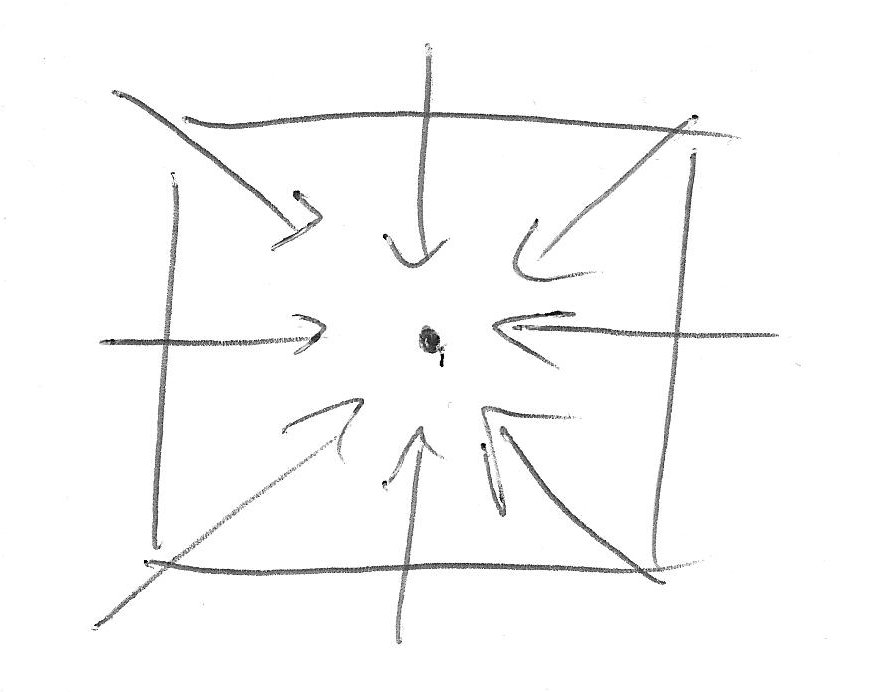
\includegraphics[width=0.4\textwidth]{img-4-2/conley-100-a.jpg}}
  \subfloat{
    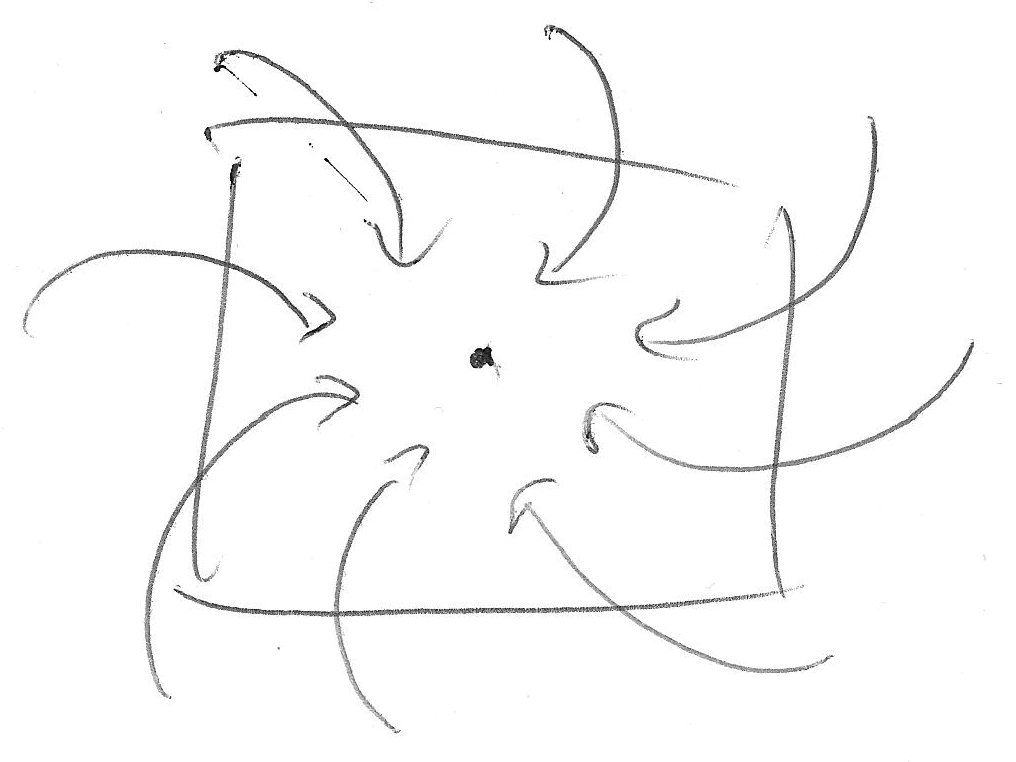
\includegraphics[width=0.4\textwidth]{img-4-2/conley-100-b.jpg}}
  \caption{vector fields for Conley index $\beta_0 = 1$, $\beta_1 = 0$ and
$\beta_2 = 0$}
  \label{fig:conley-100}
\end{figure}

\subsection*{1, 1, 0}

An attractive periodic orbit has an index of $(1, 1, 0)$ and might induce some
curl, see fig. \ref{fig:conley-110}.

\begin{figure}
  \centering
  \subfloat{
    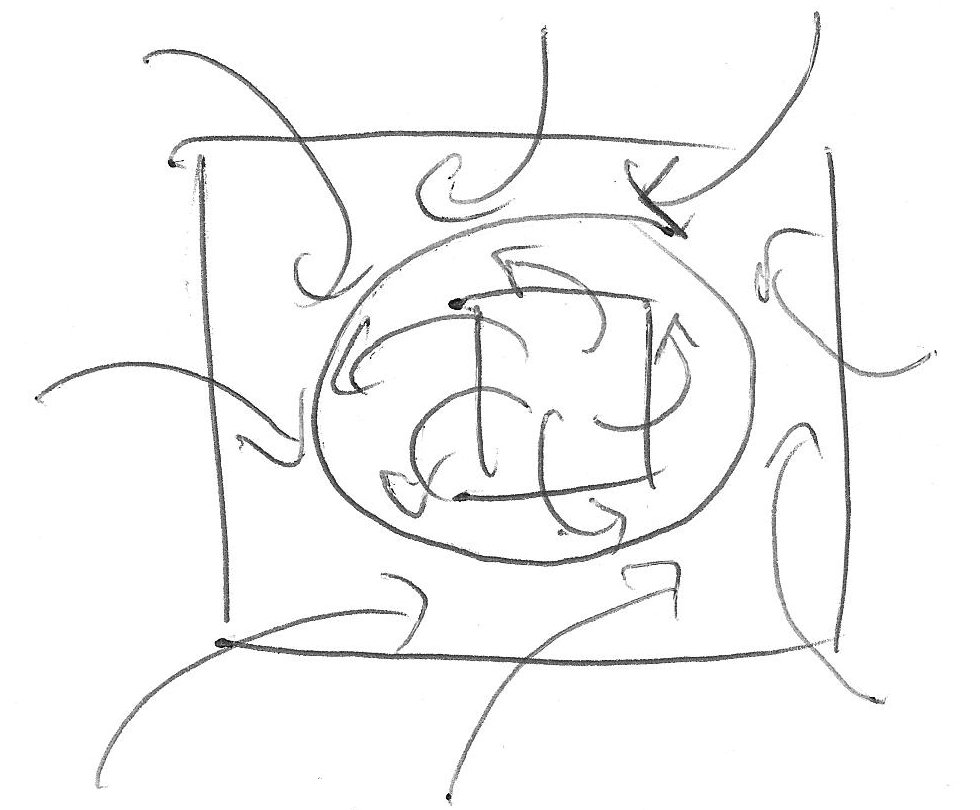
\includegraphics[width=0.4\textwidth]{img-4-2/conley-110-a.jpg}}
  \subfloat{
    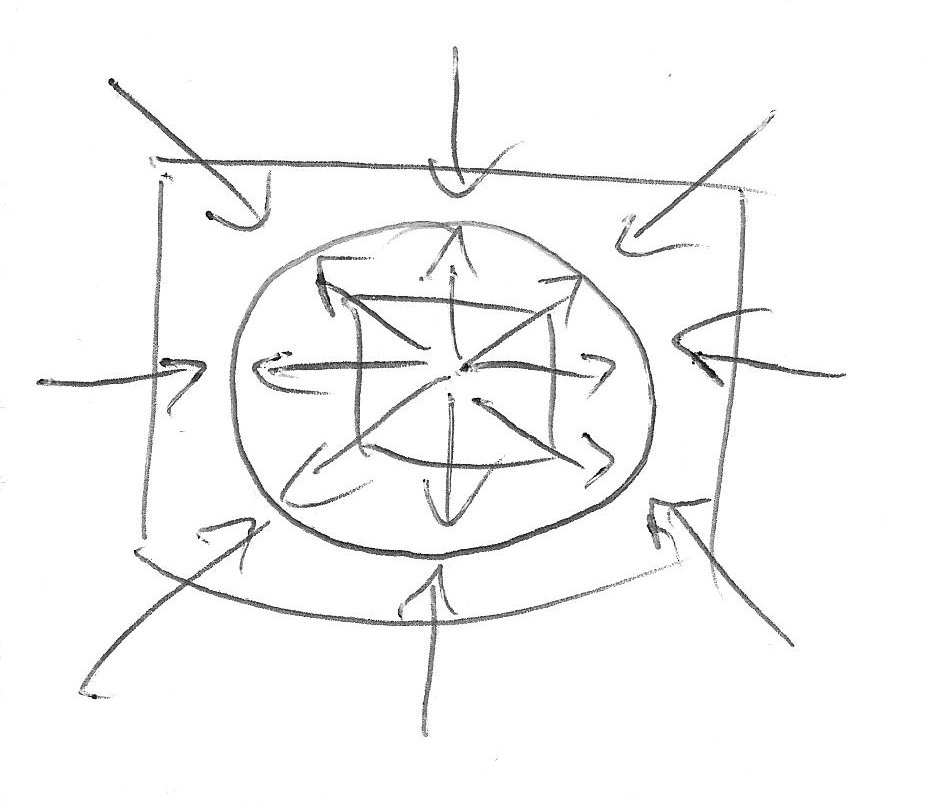
\includegraphics[width=0.4\textwidth]{img-4-2/conley-110-b.jpg}}
  \caption{vector fields for Conley index $\beta_0 = 1$, $\beta_1 = 1$ and
$\beta_2 = 0$}
  \label{fig:conley-110}
\end{figure}

\subsection*{0, 2, 1}

I assume we can add two repulsive periodic orbits such that they create a field
whose combined conley-index is $(0,2,1)$. See also fig. \ref{fig:conley-021}.

\begin{figure}
  \centering
  \subfloat{
    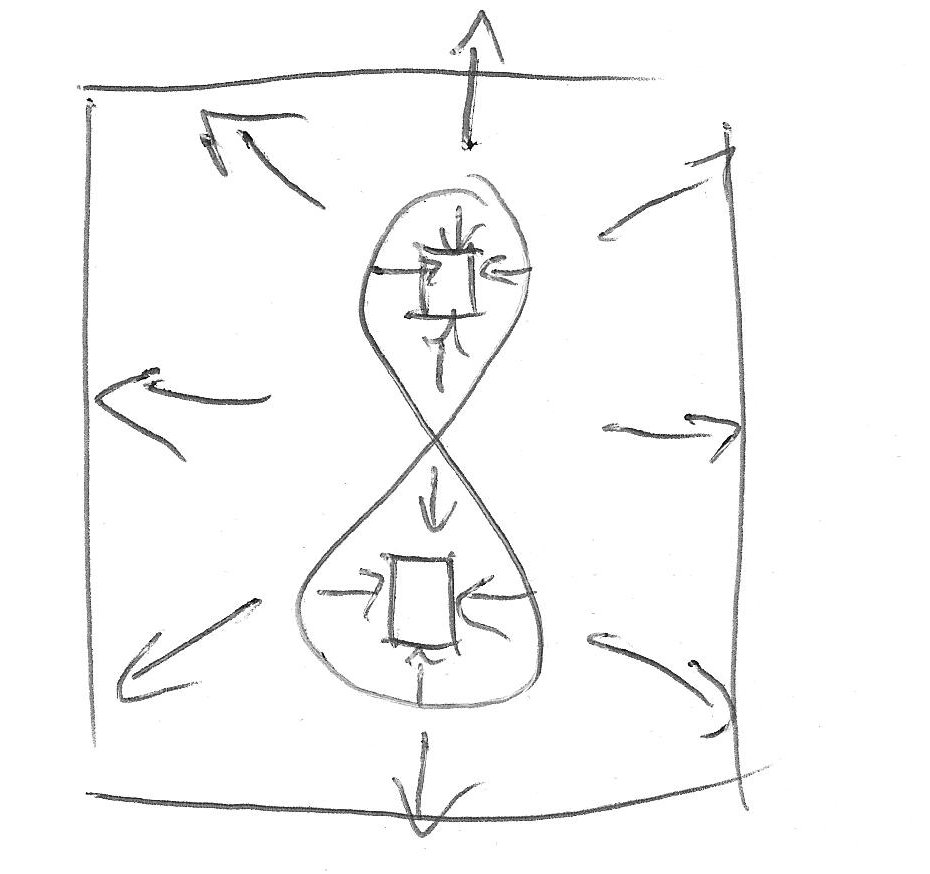
\includegraphics[width=0.4\textwidth]{img-4-2/conley-021-a.jpg}}
  \subfloat{
    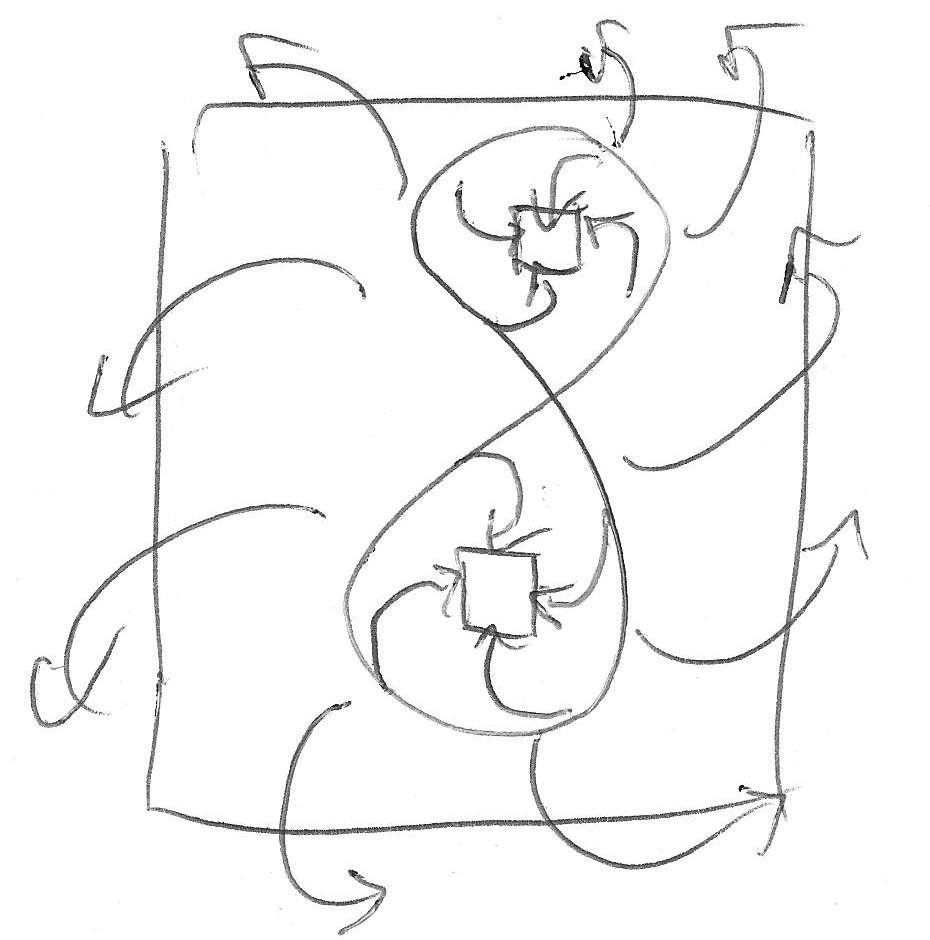
\includegraphics[width=0.4\textwidth]{img-4-2/conley-021-b.jpg}}
  \caption{vector fields for Conley index $\beta_0 = 0$, $\beta_1 = 2$ and
$\beta_2 = 1$}
  \label{fig:conley-021}
\end{figure}

\subsection*{0, 3, 0}

Again, we should be able to superimpose three saddles to create an octupole
with a conley index of $(0, 3, 0)$. See fig. \ref{fig:conley-030}.

\begin{figure}
  \centering
  \subfloat{
    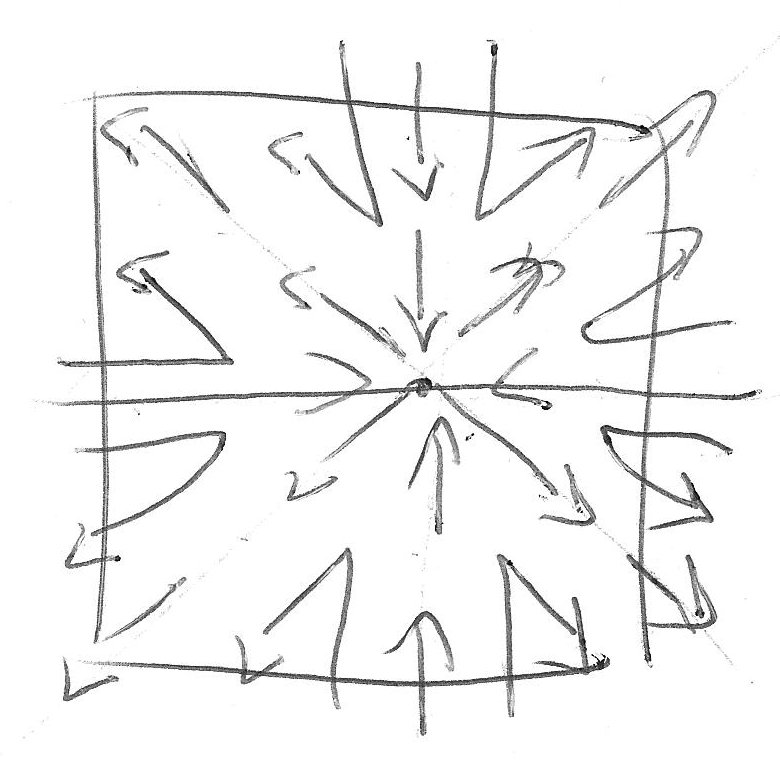
\includegraphics[width=0.4\textwidth]{img-4-2/conley-030-a.jpg}}
  \subfloat{
    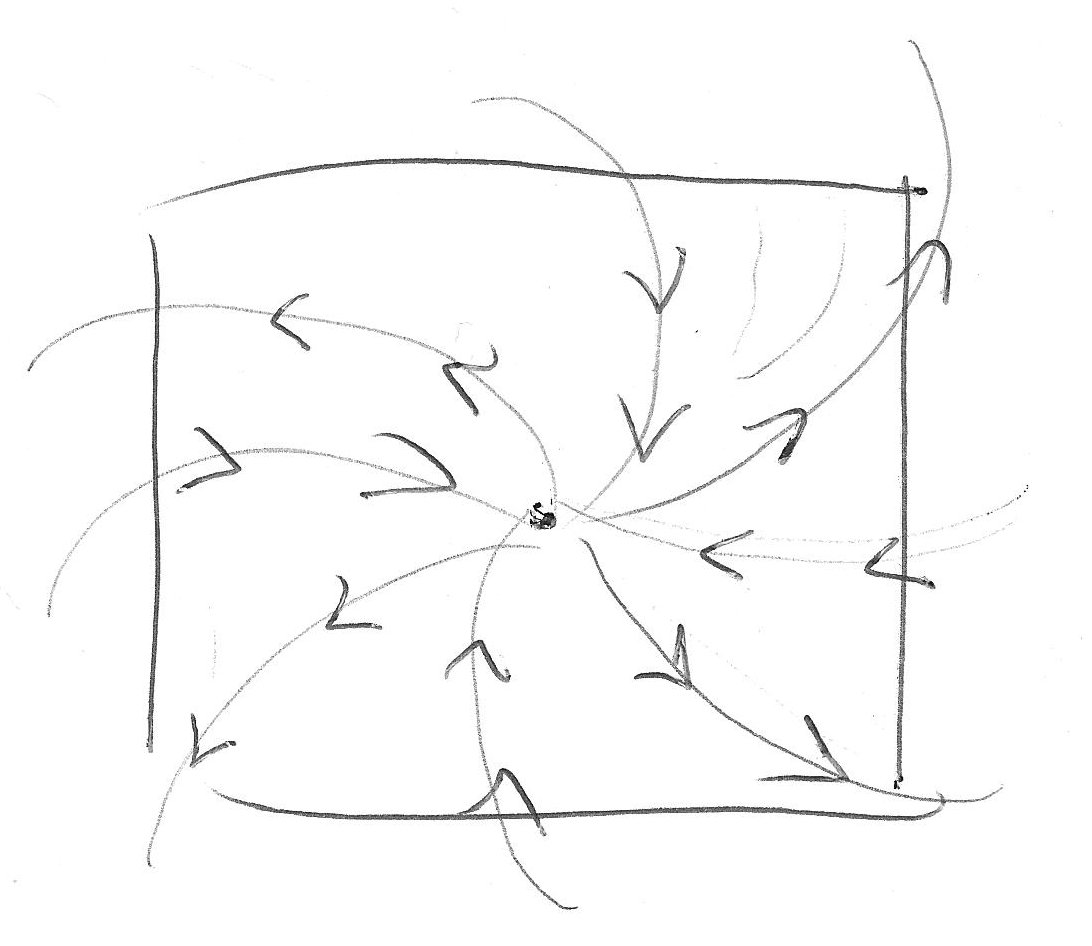
\includegraphics[width=0.4\textwidth]{img-4-2/conley-030-b.jpg}}
  \caption{vector fields for Conley index $\beta_0 = 0$, $\beta_1 = 3$ and
$\beta_2 = 0$}
  \label{fig:conley-030}
\end{figure}

\section{Tensor Field Design}

Our programming task consisted this time of adapting our previous vector field
design application to visualize symmetric second order tensor fields. We
followed the algorithms and ideas outlined by Zhang, Hays and Turk in
\cite{tfd}.

A screenshot of my implementation can be found in fig. \ref{fig:tfd-app}.

\begin{figure}
 \centering
 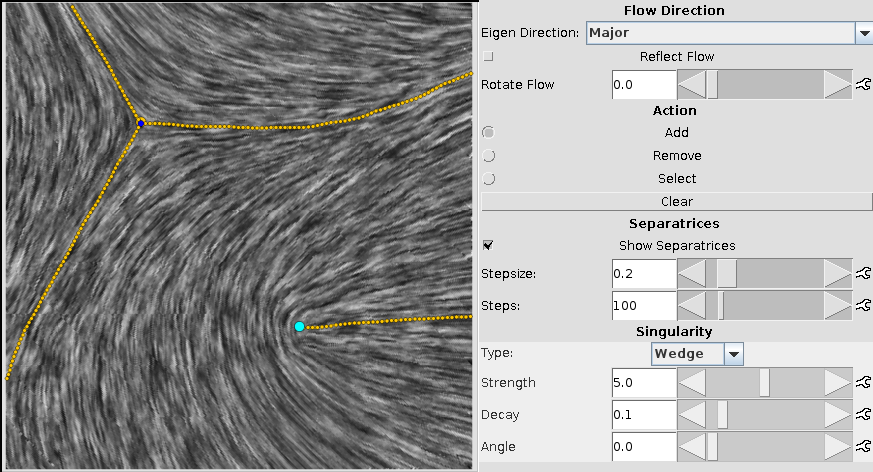
\includegraphics[scale=0.5]{img-4-2/app.png}
 \caption{Tensor Field Design Application}
 \label{fig:tfd-app}
\end{figure}

\subsection{Design Elements}

The application allows the user to interactively create a tensor field. You
choose one of six design elements (see fig. \ref{fig:tfd-elements} and
\cite{tfd}~p.~99f) and then click into the view space to place it. The
elements can be moved by drag and drop or be removed again as well.

The total second order tensor field is then defined through

\begin{equation}
 \mat{T}(\vec{r}) = \sum_i^N \mat{T}_i(\vec{r}).
 \label{eq:tf}
\end{equation}

The class \texttt{TensorField} and the inheritors classes of
\texttt{TensorTerm} provide the code implementation of this.

\begin{figure}
  \centering
  \subfloat[constant]{
    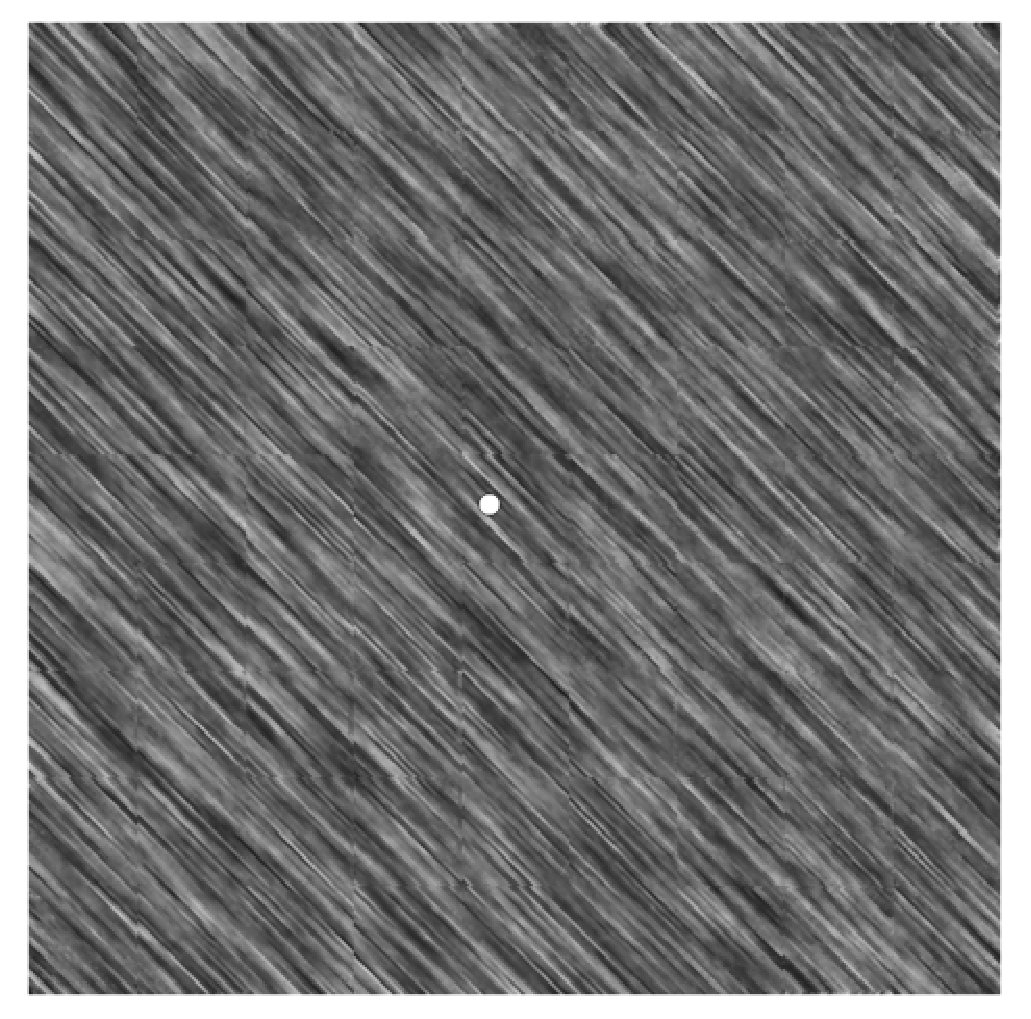
\includegraphics[width=0.3\textwidth]{img-4-2/constant.eps}}
  \subfloat[wedge]{
    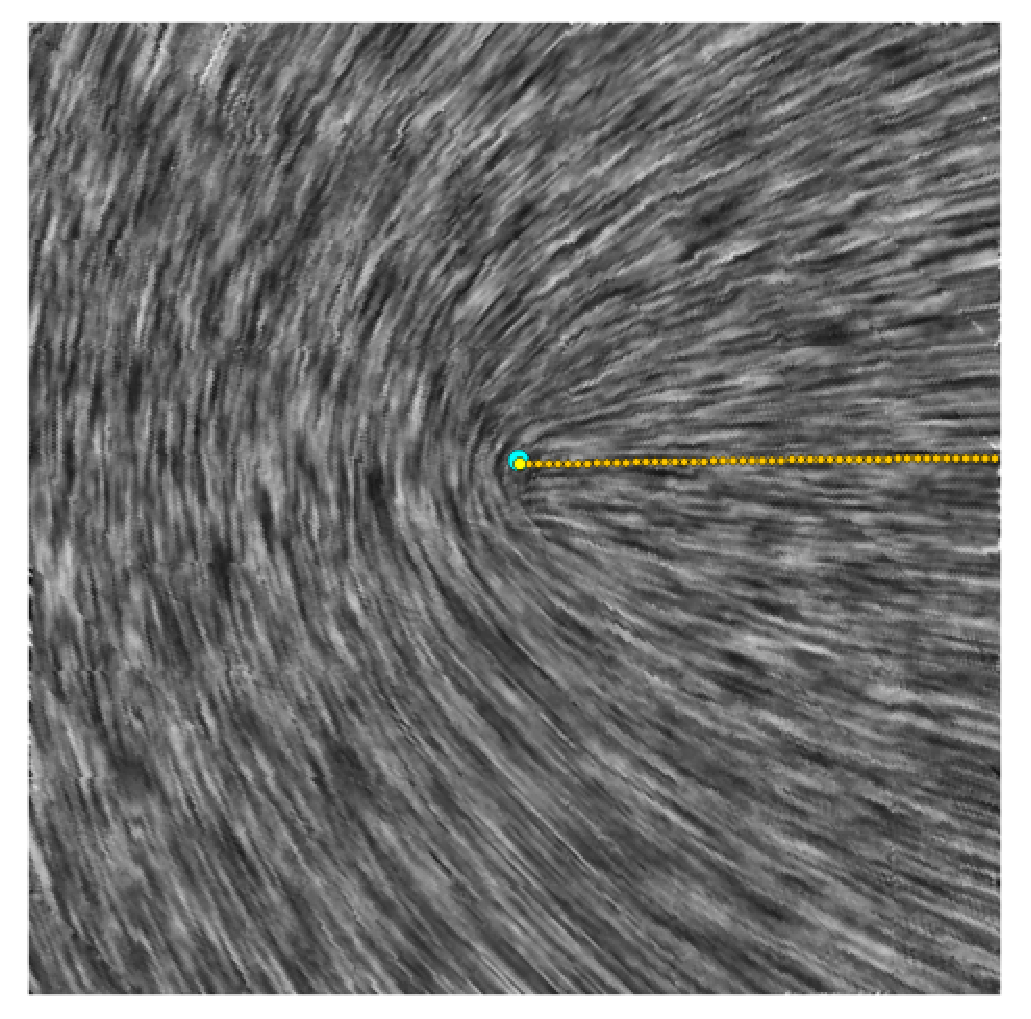
\includegraphics[width=0.3\textwidth]{img-4-2/wedge-s.eps}}
  \subfloat[trisector]{
    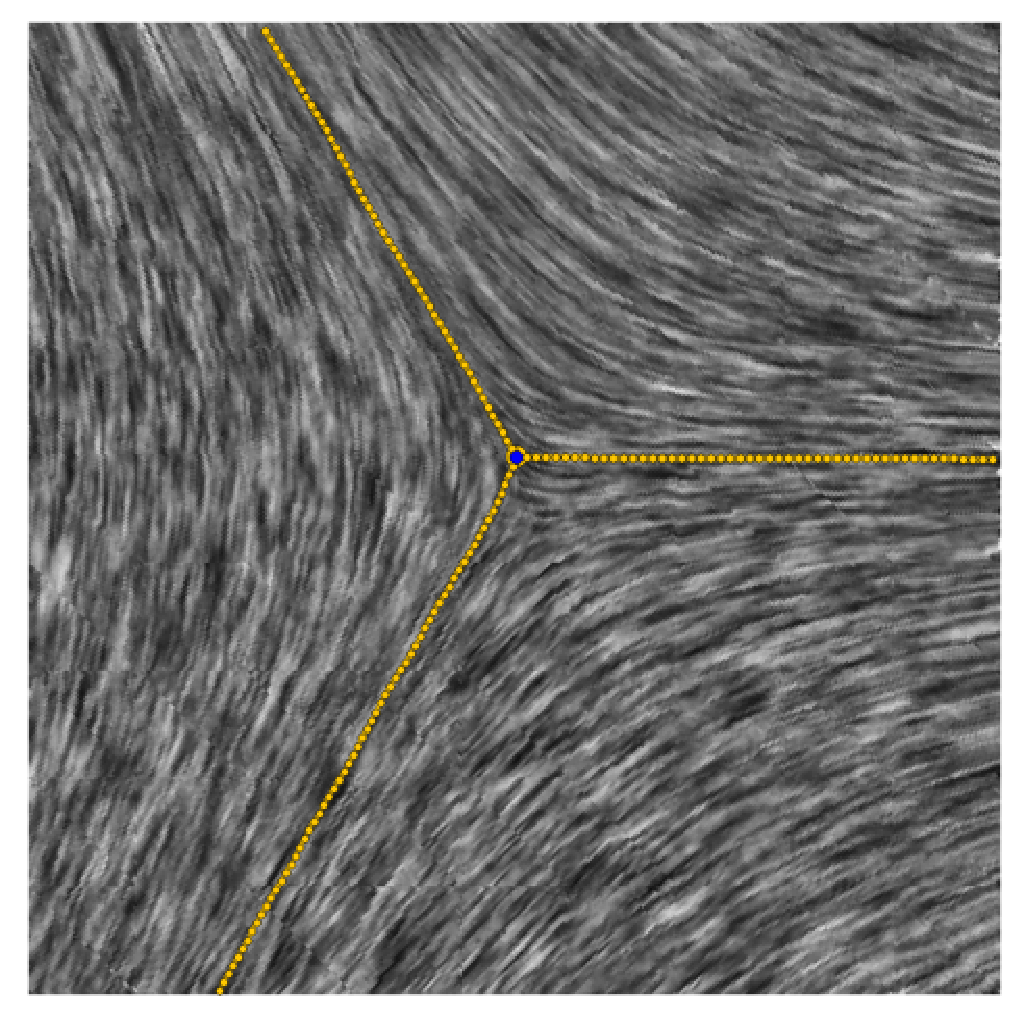
\includegraphics[width=0.3\textwidth]{img-4-2/trisector-s.eps}}
  \\
  \subfloat[node]{
    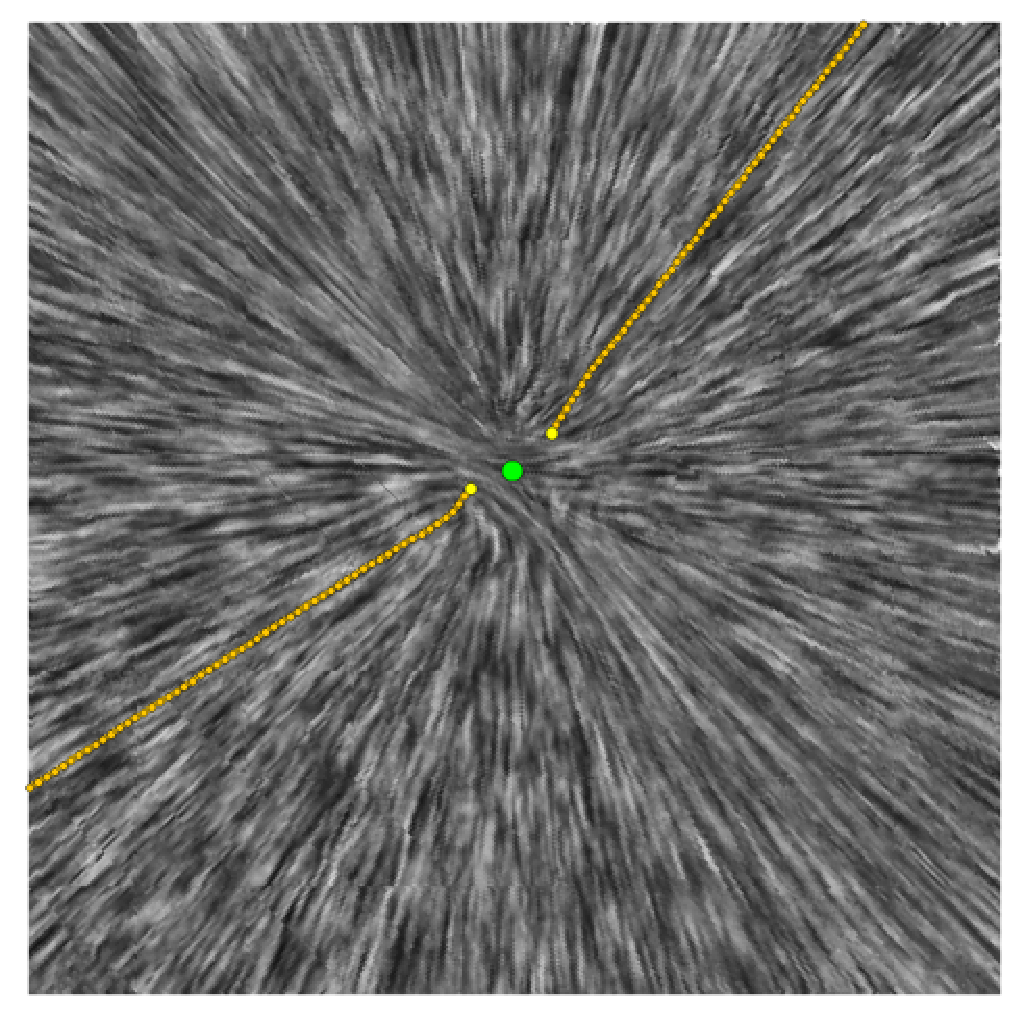
\includegraphics[width=0.3\textwidth]{img-4-2/node-s.eps}}
  \subfloat[center]{
    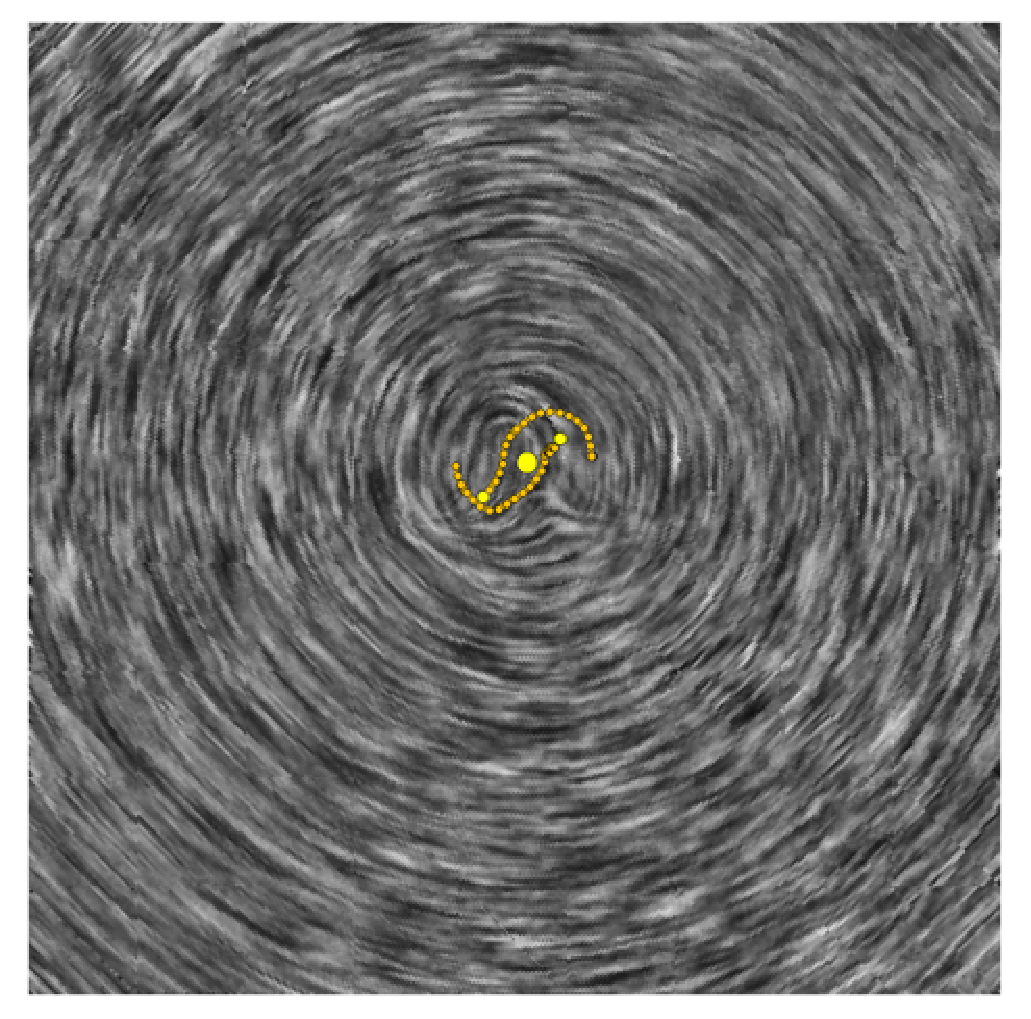
\includegraphics[width=0.3\textwidth]{img-4-2/center-s.eps}}
  \subfloat[saddle]{
    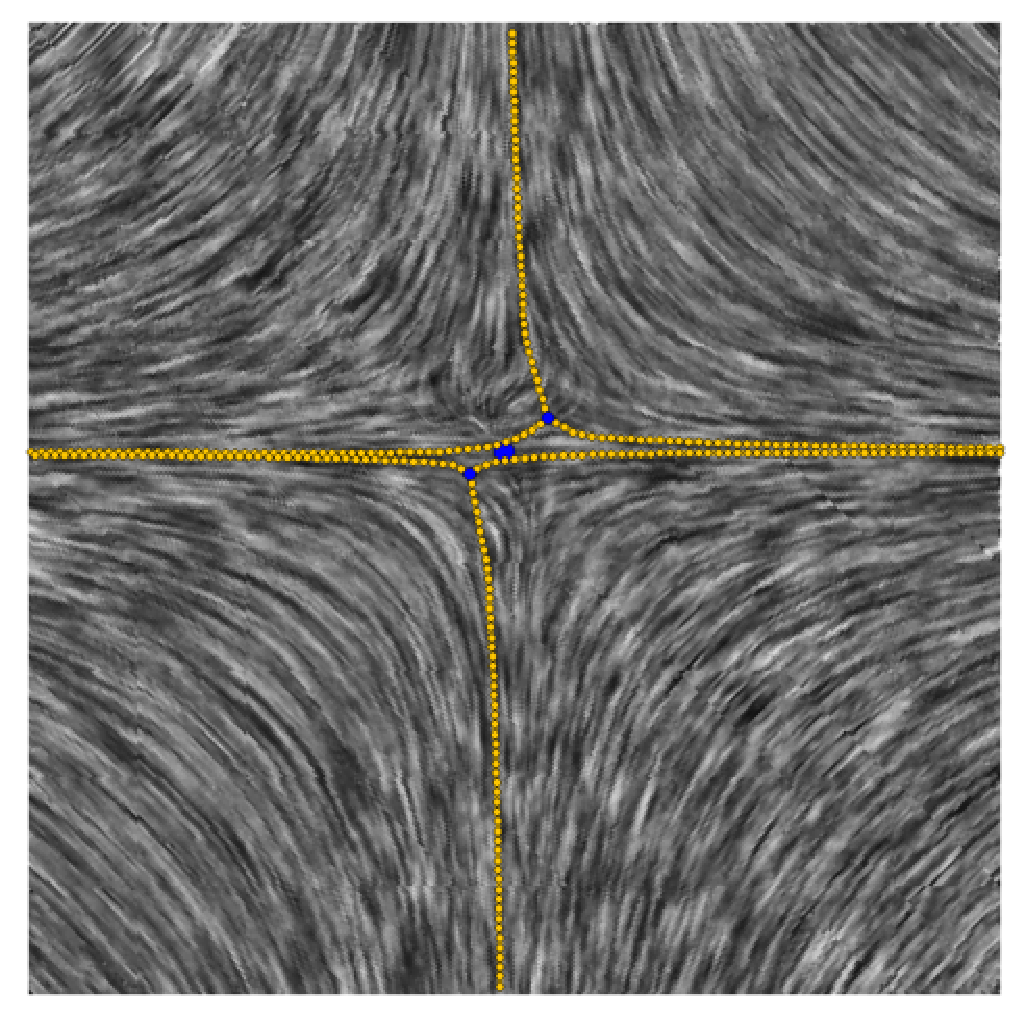
\includegraphics[width=0.3\textwidth]{img-4-2/saddle-s.eps}}
  \caption{tensor field design elements}
  \label{fig:tfd-elements}
\end{figure}

\newpage

\subsection{Rotation and Reflection}

To rotate the tensor field by an angle $\theta$, we use the reflection matrix

\begin{equation}
 \mat{R} = \left( \begin{array}{cc}
            \cos(\theta/2) & -\sin(\theta/2) \\
            \sin(\theta/2) & \cos(\theta/2) \end{array}
\right)
\end{equation}

The rotated tensor field is then obtained from eq. \ref{eq:tf} using

\begin{equation}
 \mat{T}'(\vec{r}) = \mat{R} \mat{T}(\vec{r}) \mat{R}^T.
\end{equation}

To additionally reflect the tensor field along the axis defined by $\theta$, we
can use a reflection matrix $\mat{R}'$ instead of $\mat{R}$:

\begin{equation}
 \mat{R}' = \left( \begin{array}{cc}
            \cos(\theta/2) & \sin(\theta/2) \\
            \sin(\theta/2) & -\cos(\theta/2) \end{array}
\right)
\end{equation}

Take a look at fig. \ref{fig:tfd-rotation} for tensor field rotation and at
fig. \ref{fig:tfd-reflection} for tensor field reflection.

\begin{figure}
  \centering
  \subfloat[original]{
    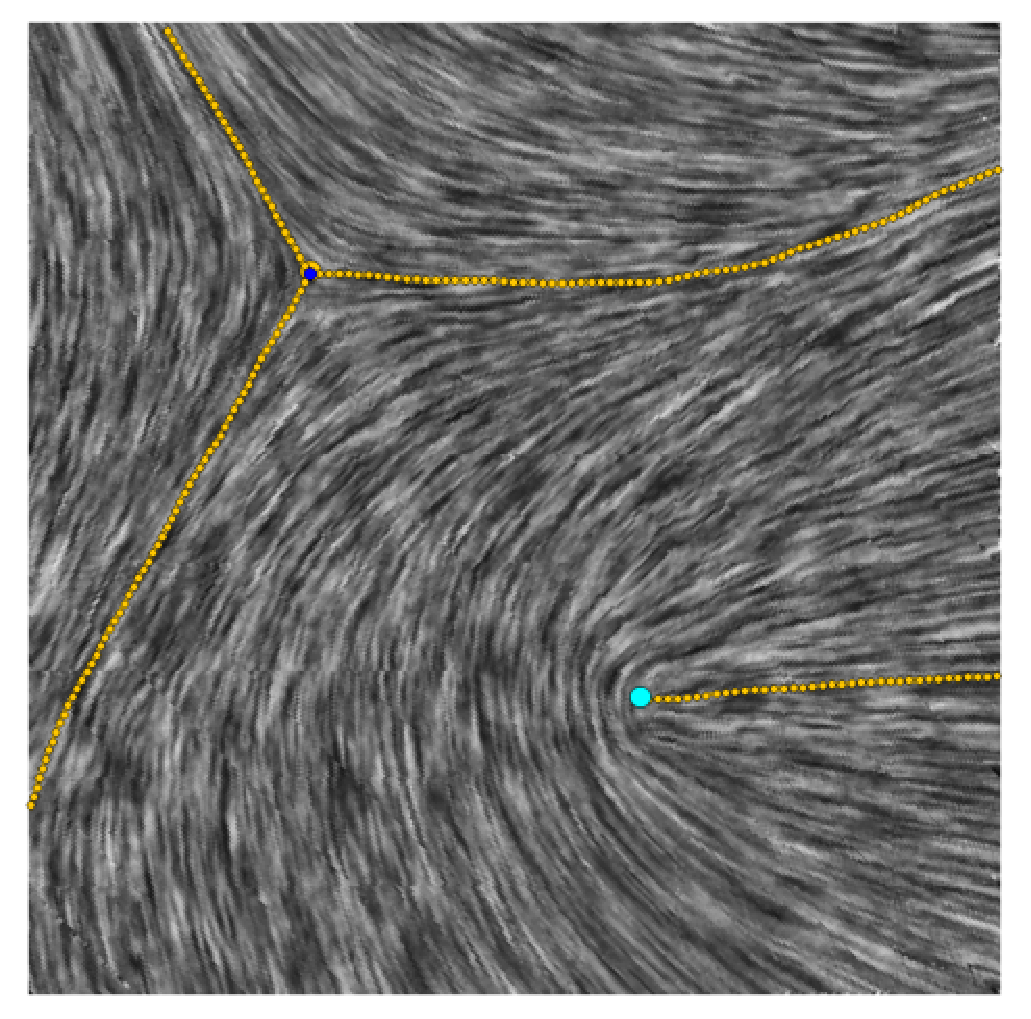
\includegraphics[width=0.3\textwidth]{img-4-2/wedge-trisector-base.eps}}
  \subfloat[$45\degree$ rotation]{
    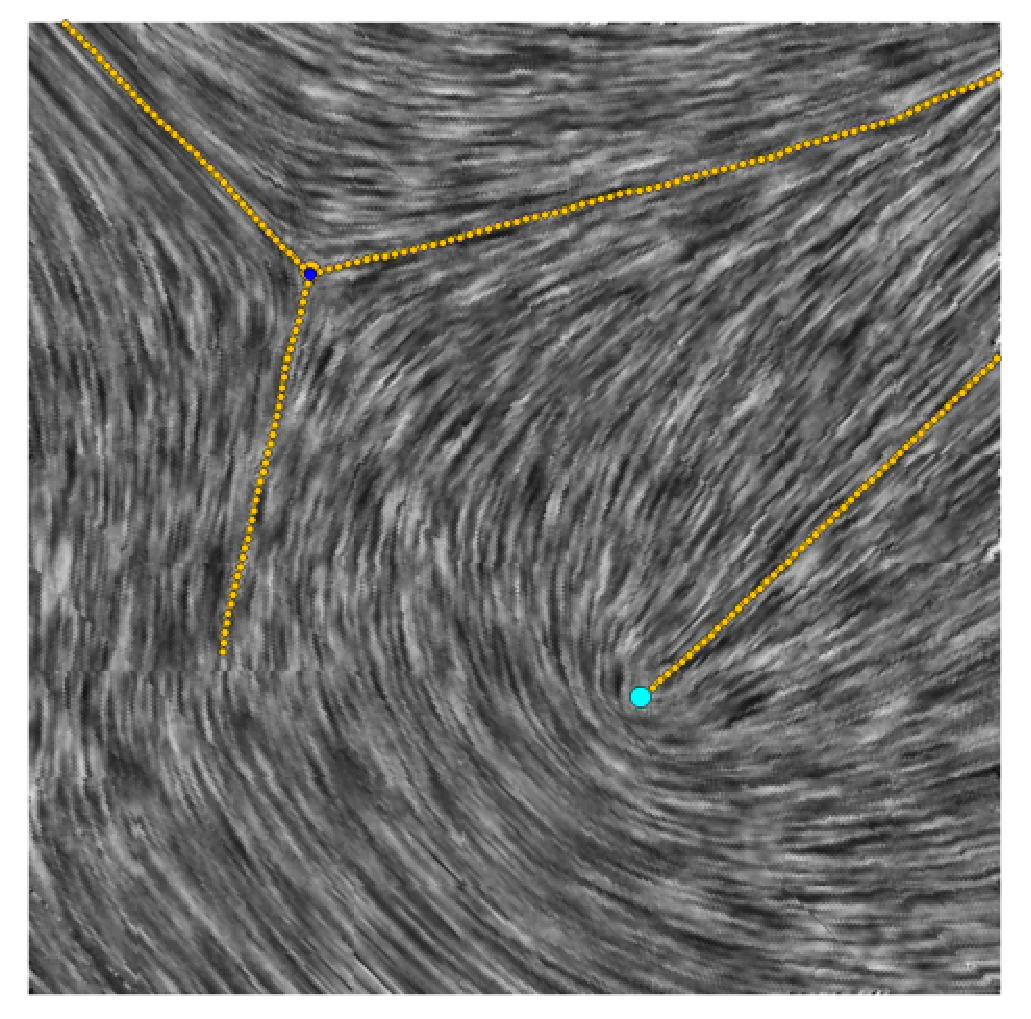
\includegraphics[width=0.3\textwidth]{img-4-2/wedge-trisector-45.eps}}
  \subfloat[$90\degree$ rotation]{
    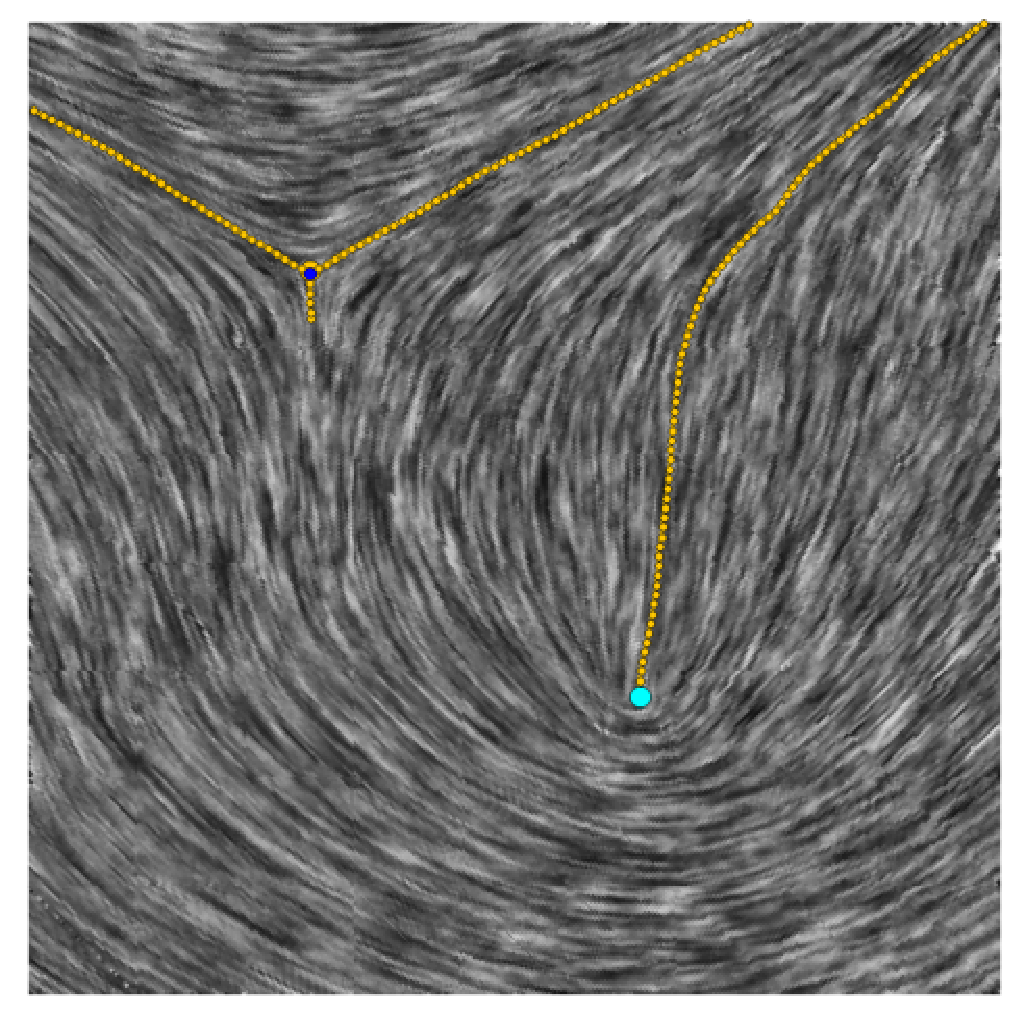
\includegraphics[width=0.3\textwidth]{img-4-2/wedge-trisector-90.eps}}
  \\
  \subfloat[$135\degree$ rotation]{
    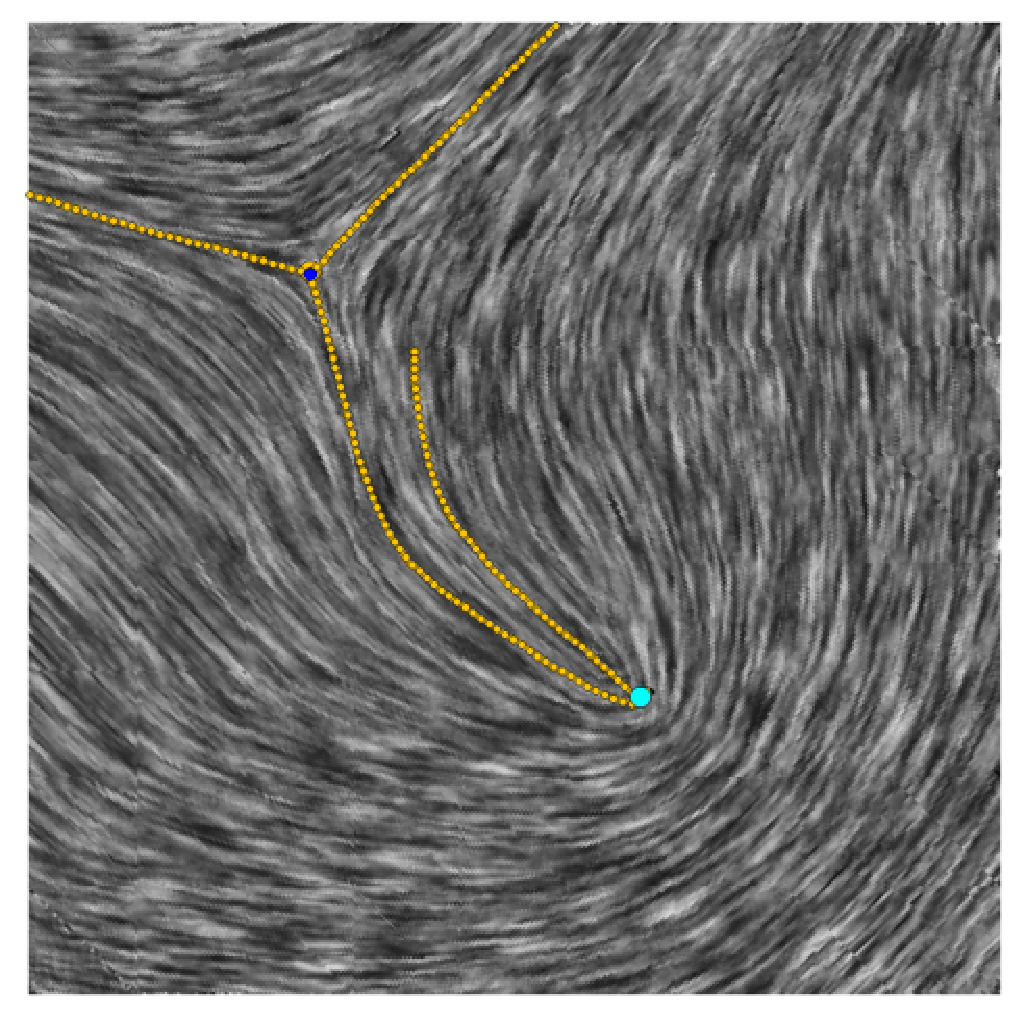
\includegraphics[width=0.3\textwidth]{img-4-2/wedge-trisector-135.eps}}
  \subfloat[$180\degree$ rotation]{
    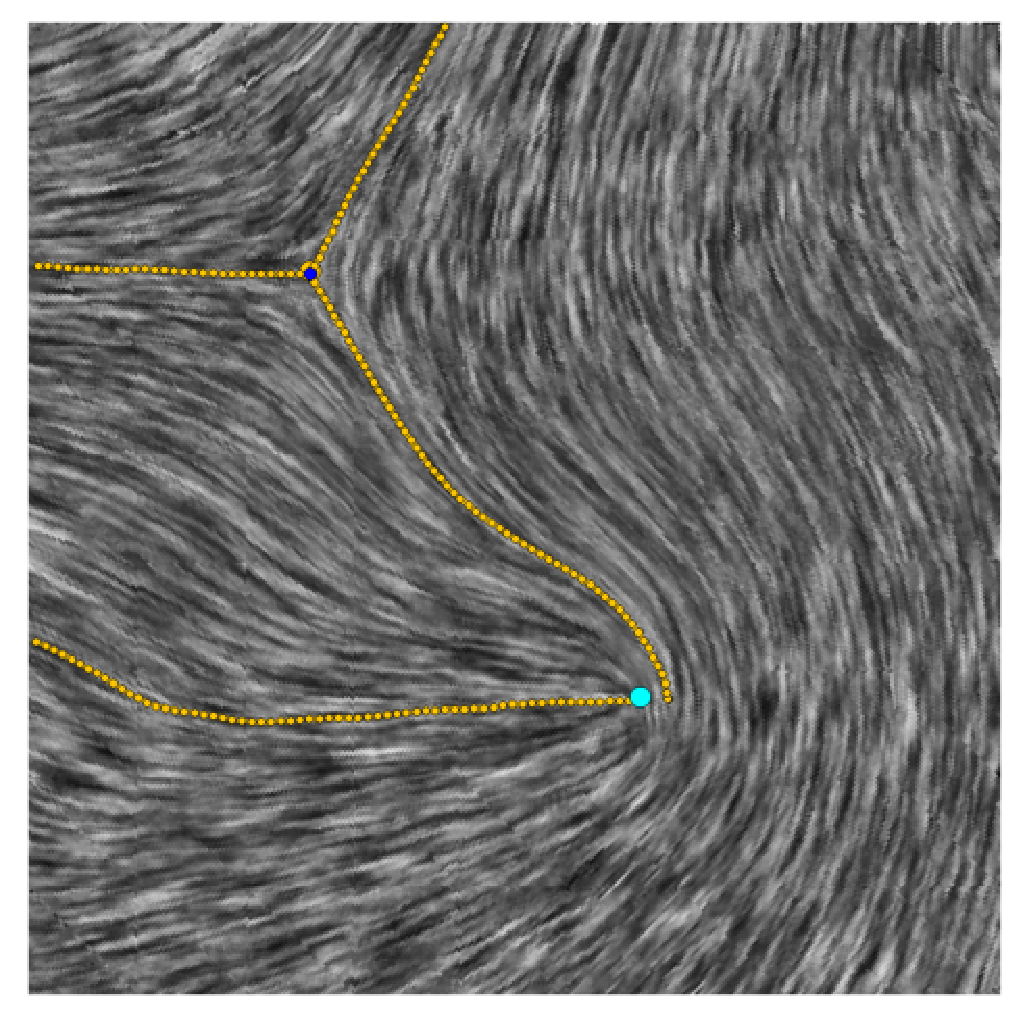
\includegraphics[width=0.3\textwidth]{img-4-2/wedge-trisector-180.eps}}
  \subfloat[$270\degree$ rotation]{
    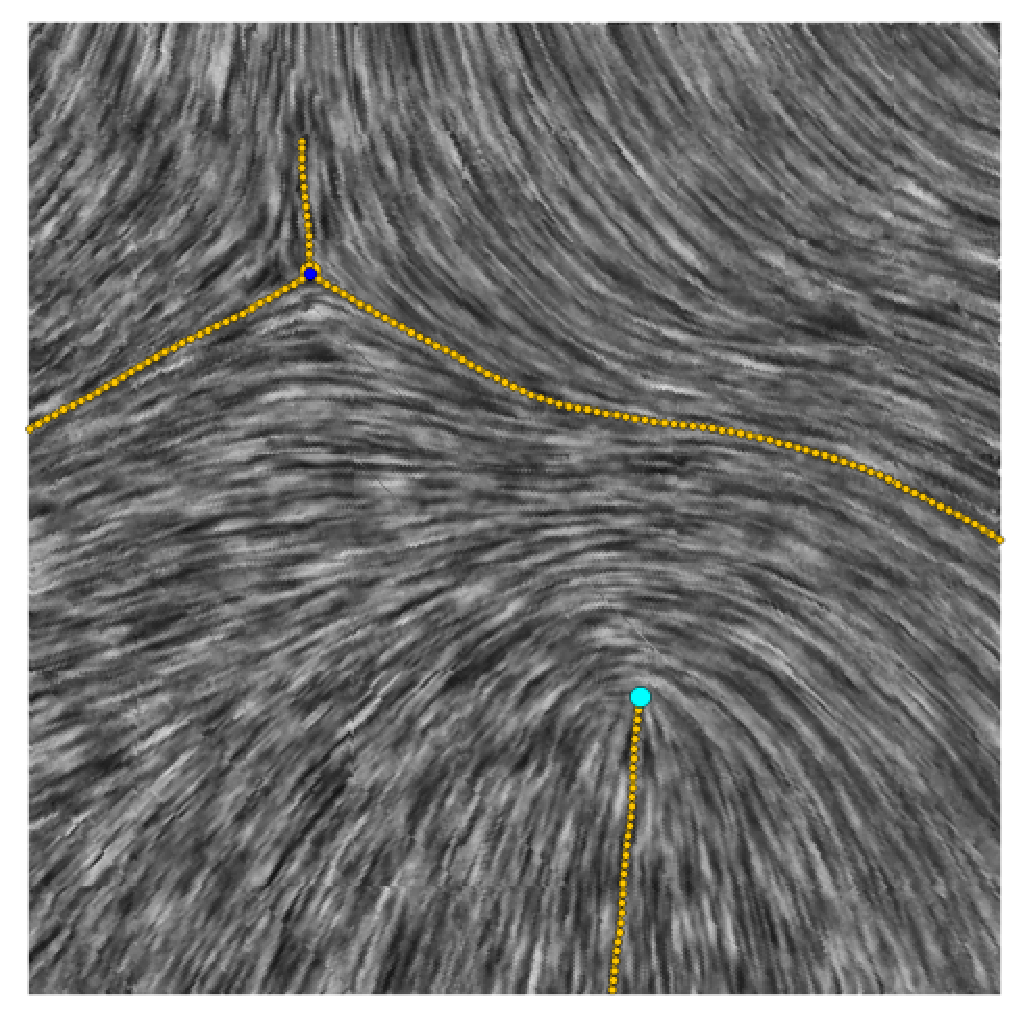
\includegraphics[width=0.3\textwidth]{img-4-2/wedge-trisector-270.eps}}
  \caption{tensor field rotation}
  \label{fig:tfd-rotation}
\end{figure}

\begin{figure}
  \centering
  \subfloat[original]{
    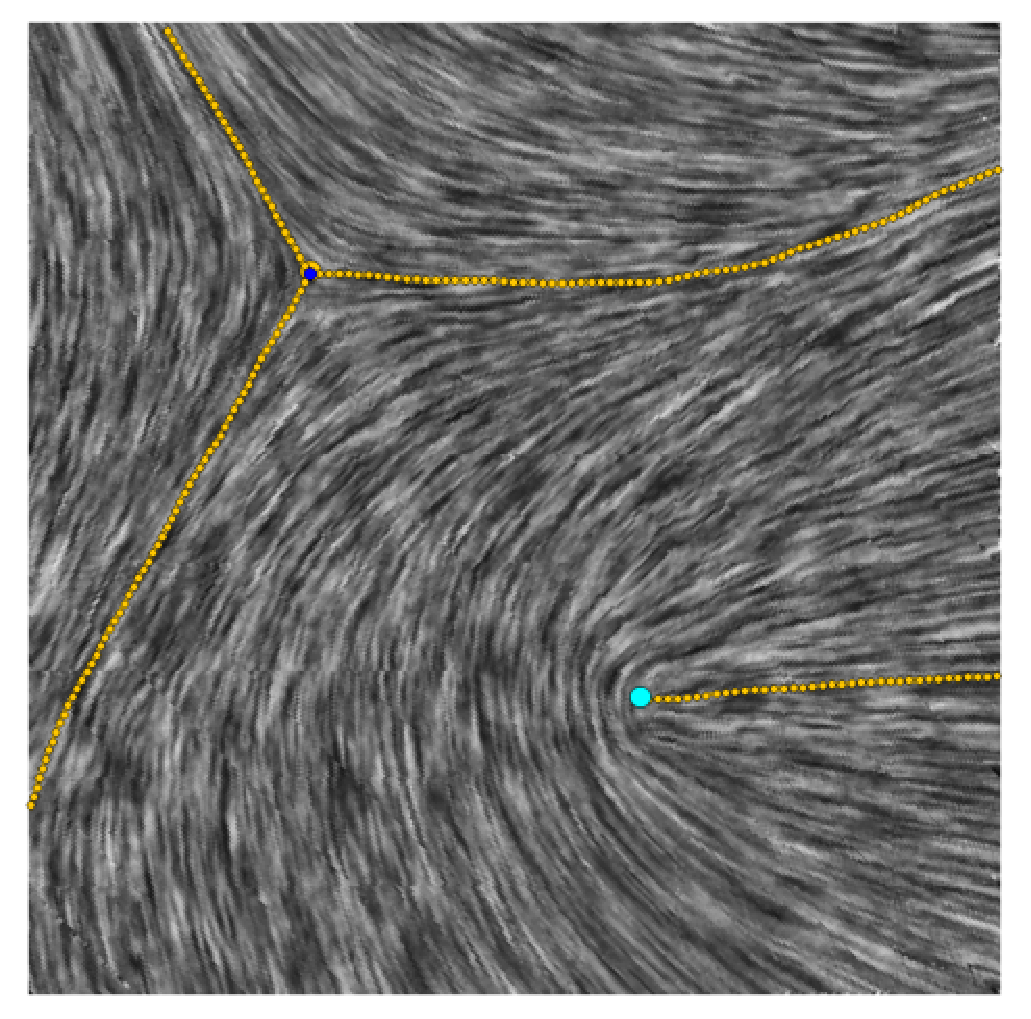
\includegraphics[width=0.4\textwidth]{img-4-2/wedge-trisector-base.eps}}
  \subfloat[reflected]{
    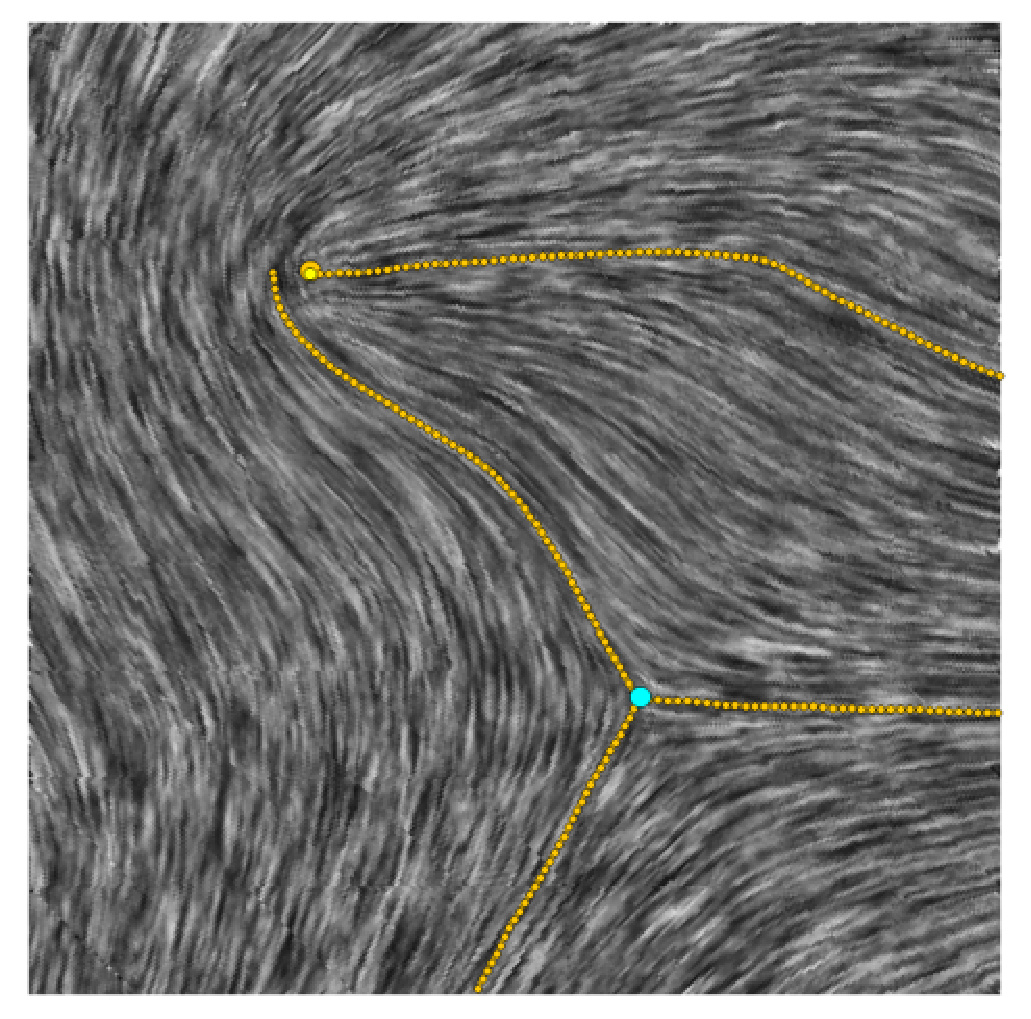
\includegraphics[width=0.4\textwidth]{img-4-2/wedge-trisector-reflect.eps}
  }
  \caption{tensor field reflection}
  \label{fig:tfd-reflection}
\end{figure}

\subsection{Discretization and Interpolation}

The continous tensor field in eq. \ref{eq:tf} must be discretized for numerical
analysis and visualization. First, we use a triangulated domain and compute the
tensor field at each vertex. Then we interpolate the tensor field in each
triangle from the three fields  $\mat{T}_{1,2,3}$ at the vertices
$\vec{v}_{i} = (x_i,y_i)$, $i = 1,2,3$, by solving the two equation systems

\begin{equation}
 \left ( \begin{array}{c c c}
          a/c & b/d & c/f \\
          x_1 & y_1 & 1 \\
          x_2 & y_2 & 1 \\
          x_3 & y_3 & 1
         \end{array}
         \right \rvert
 \left .
      \begin{array}{c c}
      \alpha & \beta \\
       T_{1_{0,0}} & T_{1_{1,0}} \\
       T_{2_{0,0}} & T_{2_{1,0}} \\
       T_{3_{0,0}} & T_{3_{1,0}}
      \end{array}
 \right )
\end{equation}

yielding the symmetric second order interpolated tensor field

\begin{equation}
 \mat{T}_I(\vec{r}) = \left(\begin{array}{c c}
                       ax + by + e & cx + dy + f \\
                       cx + dy + f & -ax -by -e
                      \end{array}\right).
 \label{eq:tf-linear}
\end{equation}

Note that this interpolation is of course only valid inside the triangle
spanned by the vertices $\vec{v}_{1,2,3}$.

The class \texttt{InterpolatedTensorField} implements the interpolation scheme
outlined above.

\subsection{Eigenvector Field Visualization}

To visualize the tensor field we use the image based approach outlined in
\cite{tfd} p.~98f, which allows us to reuse the LIC code from JavaView. For the
major eigenvector field, we can directly  follow the equations outlined
there. For the minor eigenvector field though, we have to make small
adjustments: The minor eigenvector $\vec{E}_2$ is orthogonal to
$\vec{E}_1$, i.e.

\begin{equation}
 \vec{E}_2 = \left( \begin{array}{c}
              -\sin \theta \\
              \cos \theta
             \end{array} \right).
\end{equation}

We create $\vec{V}_x$ such that the $x$-component is positive:

\begin{equation}
 \vec{V}_x = \left \{  \begin{array}{l l}
                       \vec{E}_2 & \quad \text{if $-\sin \theta > 0$} \\
                       -\vec{E}_2 & \quad \text{otherwise}
                       \end{array} \right.
\end{equation}

Analogously we create $\vec{V}_y$ such that its $y$-component is positive. The
weighting factors $W_{x,y}$ use the $x$- and $y$-component of $\vec{E}_2$. Hence
they are

\begin{eqnarray}
 W_x &=& \sin^2 \theta \qquad \text{, and}\\
 W_y &=& 1 - W_x = \cos^2 \theta .
\end{eqnarray}

You can see an example of the above code in fig. \ref{fig:tfd-majorminor}. If
you are interested in the code that implements the calculations above, take a
look at \texttt{Ex4\_3.updateLICImage} and \texttt{Ex4\_3.computeWeight}.

\begin{figure}
  \centering
  \subfloat[major]{
    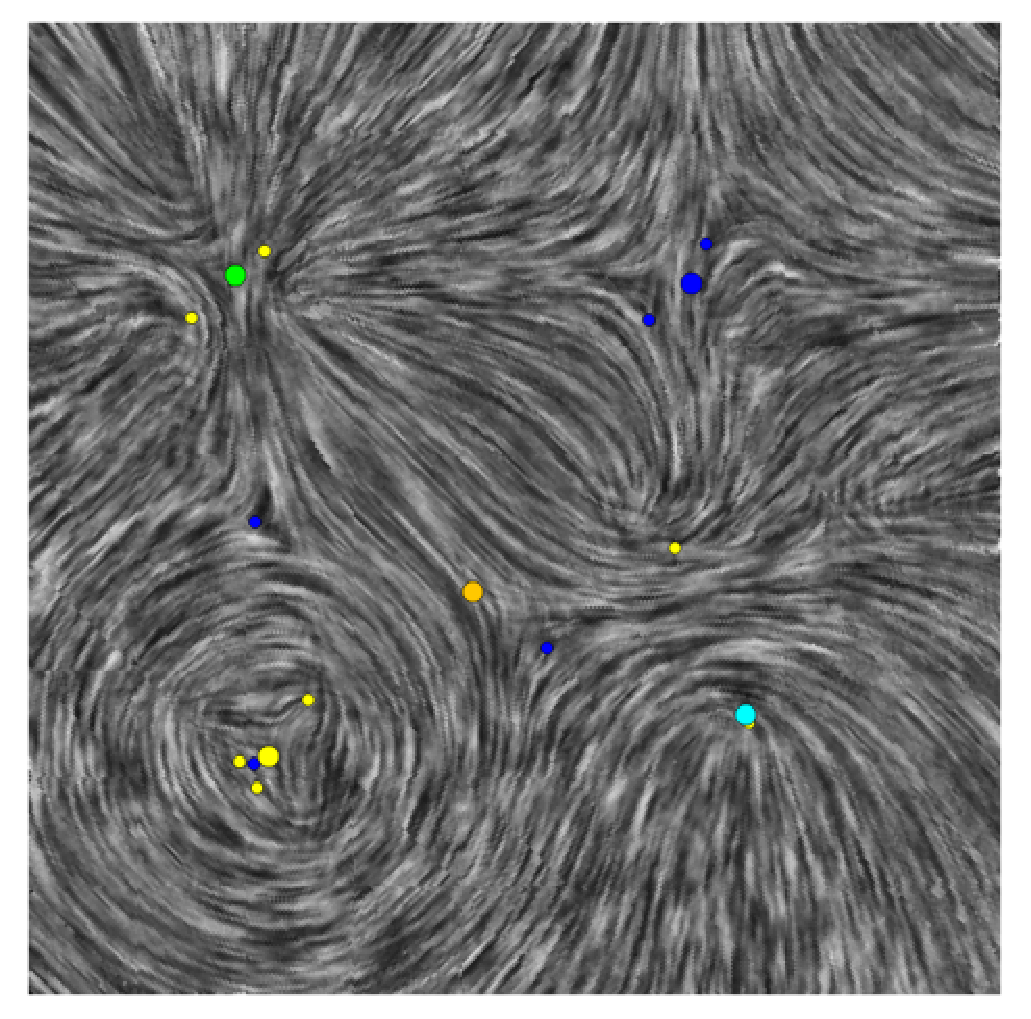
\includegraphics[width=0.4\textwidth]{img-4-2/major.eps}
    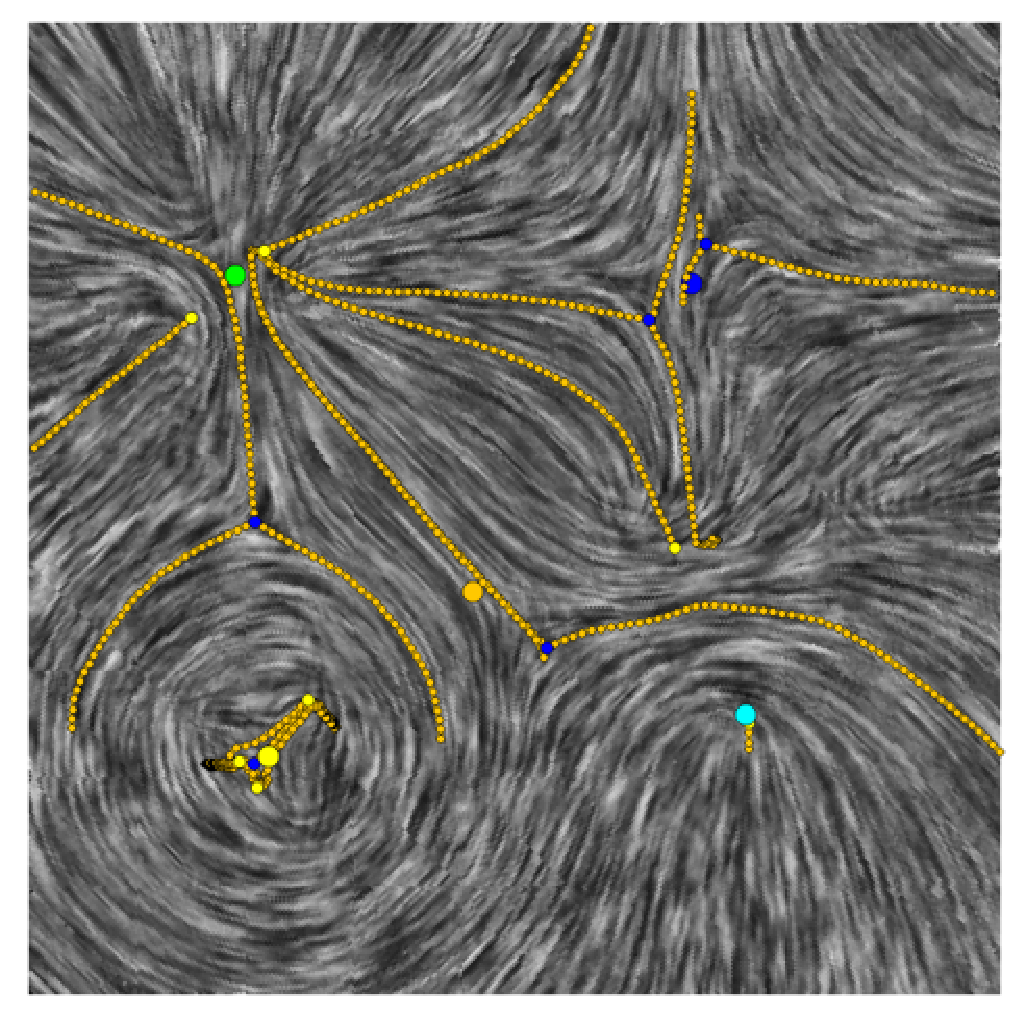
\includegraphics[width=0.4\textwidth]{img-4-2/major-s.eps}
  }
  \\
  \subfloat[minor]{
    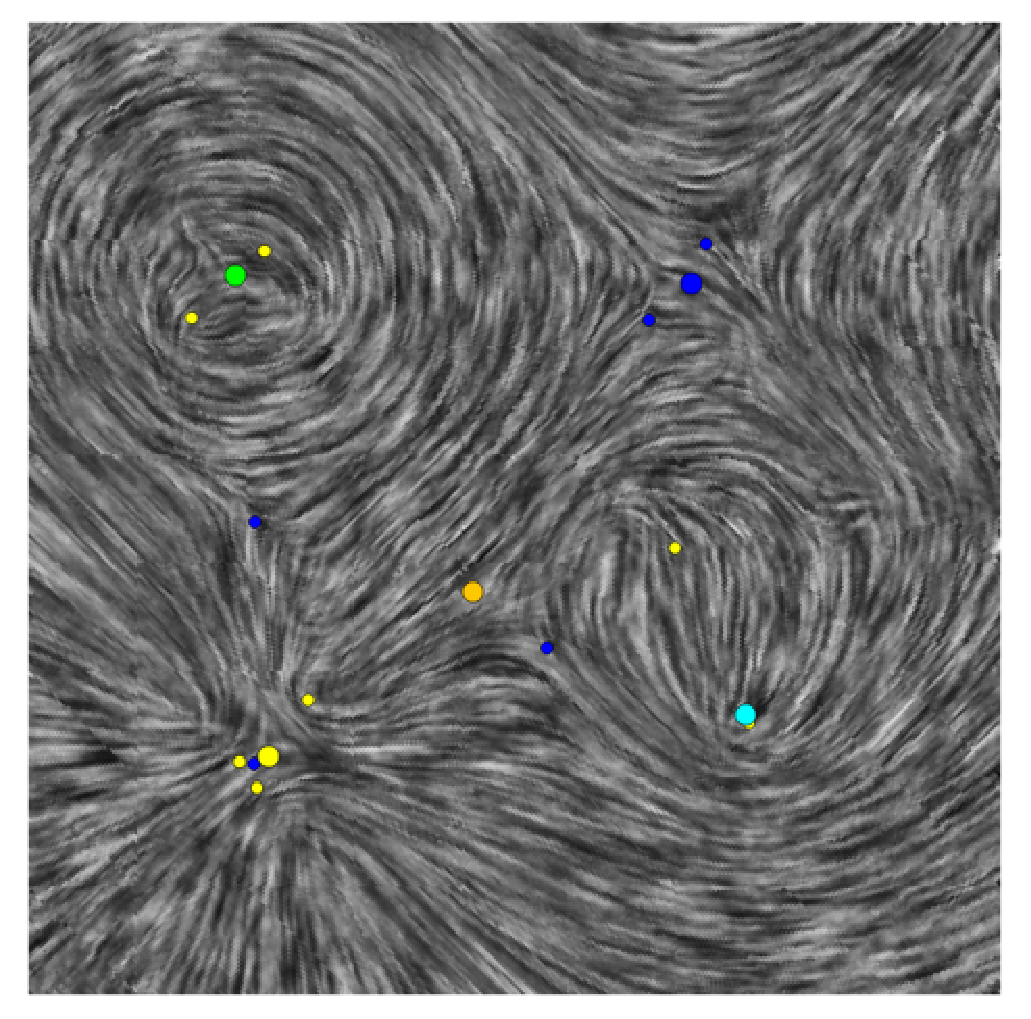
\includegraphics[width=0.4\textwidth]{img-4-2/minor.eps}
    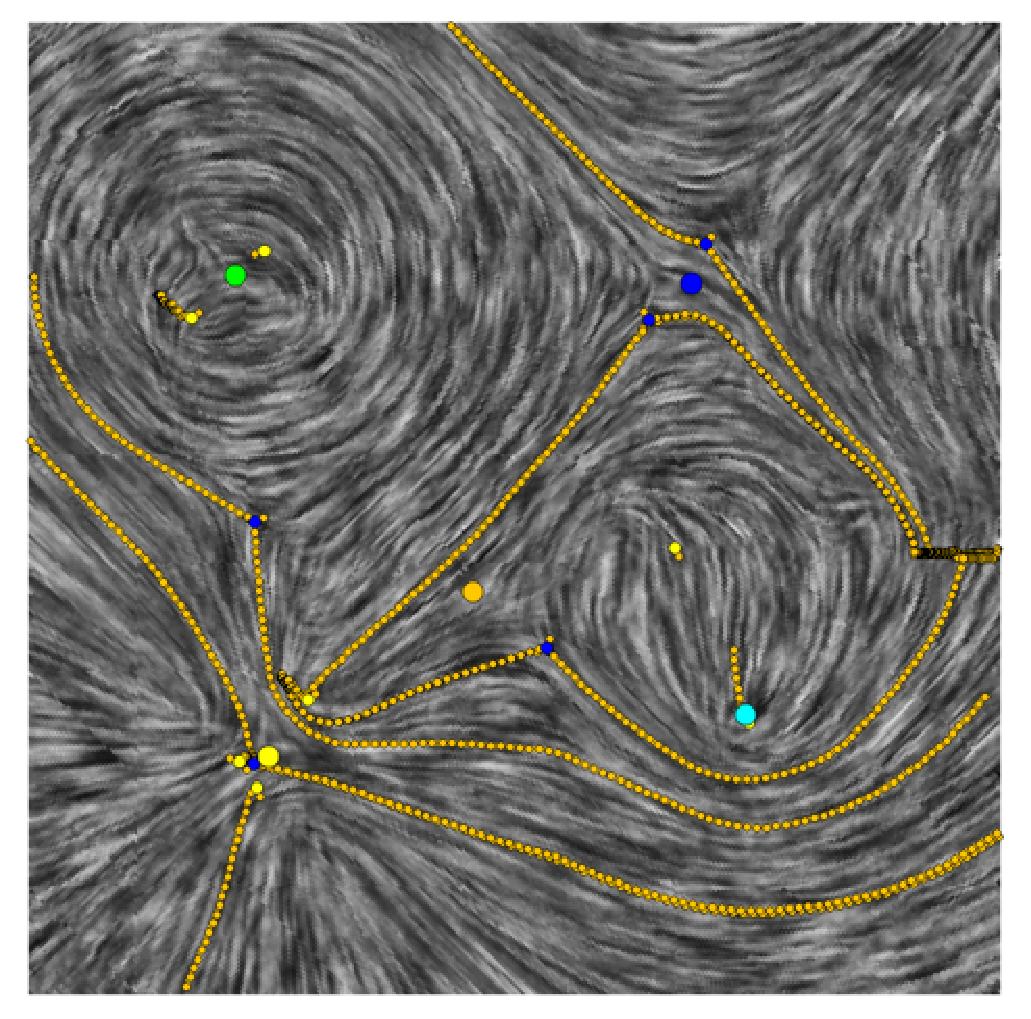
\includegraphics[width=0.4\textwidth]{img-4-2/minor-s.eps}
  }
  \caption{minor and major eigenvector fields}
  \label{fig:tfd-majorminor}
\end{figure}

\subsection{Degenerate Points}

To find the degenerate points of a symmetric second order tensor field we
iterate over all interpolated tensor fields (see eq. \ref{eq:tf-linear}) in our
domain and solve the equation system

\begin{equation}
  \left(\begin{array}{c c}
         a & b \\
         c & d
        \end{array} \right)
 \vec{r}_0 = \left( \begin{array}{c} -e \\ -f \end{array} \right).
\end{equation}

If $\vec{r}_0$ lies in the triangle for which the interpolation is valid, then
we found a degenerate point. We can furthermore classify it by calculating the
determinant of the coefficient matrix in the equation above. The degenerate
point is a wedge if the determinant is positive, a trisector if it is negative
and a higher-order degenerate point if the determinant is zero.

You can see the results of this algorithm in the figures of this report, e.g.
fig. \ref{fig:tfd-majorminor}. Wedges are represented by small yellow dots,
while trisectors are blue. Higher-order terms are usually not found, but if so
they would be colored white.

\texttt{InterpolatedTensorField.findDegeneratePoints} implements the above.

\subsection{Separatrices}

Another important feature of the tensor topology beside the degenerate points
are the separatrices. Following the scheme that was shown to us in-class we can
extract the directions of the separatrices at a wedge or trisector, by finding
the roots of the cubic polynomial

\begin{equation}
 d u^3 + (c+2b)u^2 + (2a-d)u -c = 0, \qquad \text{with $u = tan\theta$}.
\end{equation}

The coefficients $a$, $b$, $c$ and $d$ are again those from eq.
\ref{eq:tf-linear}. Solving the equation yields up to three real-valued roots
$u$. It has to be noted that the algorithm applied is not very numerically
stable and hence imaginary parts below a threshold of $1E-6$ are ignored. For
each value of $u$ we can then find two values of $\theta$. Again it can be
observed that the $atan$ calculation is very unreliably for expected values
near $90\degree$ or $270\degree$.

To figure out whether a given $\theta$ points into a minor or major direction,
we compare the eigen values, i.e.

\begin{eqnarray}
 \lambda_1 &=& \mat{T}_I(\vec{r}_0 + \vec{e}_\theta) \vec{e}_\theta \cdot
\vec{e}_\theta \\
 \lambda_2 &=& \mat{T}_I(\vec{r}_0 + \vec{e}_\theta) \vec{e}_{\theta+\pi/2}
\cdot
\vec{e}_{\theta+\pi/2},
\end{eqnarray}

where $\vec{e}_{\phi}$ is a unit vector in direction of an angle $\phi$:

\begin{equation}
 \vec{e}_{\phi} = \left( \begin{array}{c}
                          \cos \phi \\
                          \sin \phi
                         \end{array} \right )
\end{equation}

If now $\lambda_1 > \lambda_2$, then $\theta$ points into the direction of a
major separatrix. Otherwise it points into a minor direction. Based on this we
can start a classical Runge-Kutta line tracer in the selected direction, using
the eigenvector field direction as seed values for the integration scheme.

The above was already applied to find the separatrices (the orange lines) in the
previously shown images, see e.g. fig. \ref{fig:tfd-majorminor}. The
application allows the user to define the numer of steps and the stepsize. The
tracer stops near degenerate points, i.e. when the distance to a degenerate
point is less than one tenth of the stepsize.

The code that visualizes the separatrices of wedges and trisectors is
implemented in \texttt{Ex4\_3.findSeparatrices},
\texttt{TensorFieldFunctor} and \texttt{ClassicalRungeKuttaTracer}.

\bibliography{sources}

\end{document}

% kate: replace-tabs on;